\documentclass[12pt]{report}
\usepackage{thesis}


% Watermark
\usepackage{draftwatermark}
%\usepackage{amsmath}

% Watermark
\SetWatermarkText{\put(-200,100)
{
\includegraphics[width=0.13\textwidth,natwidth=50,natheight=50,
angle=-45]{Logo.jpg}}}

% FEBRIAN packages
\usepackage{times}
\usepackage{graphicx}
\usepackage{amsmath}
\usepackage{amssymb} % for math : \geqslant

\usepackage{url} %citation URL type
\usepackage{relsize} % for math : \mathlarger

%ben isok split: http://tex.stackexchange.com/questions/14673/pseudo-code-to-be-spread-over-multiple-pages
\usepackage{algorithm}
\usepackage{algpseudocode}
\usepackage{caption}

\usepackage[noadjust]{cite}
\graphicspath{{figures/}}

\usepackage{multicol}
\usepackage{multirow} % table multirow

\usepackage{csquotes} % For the command \enquote

% figures
\usepackage{wrapfig}

\usepackage{relsize} % for math : \mathlarger

% FEBRIAN packages

\begin{document}
\addcontentsline{toc}{chapter}{Nama Kampus Recommendation
Letter from the Thesis Advisor}
 % Letter from the Thesis Advisor: Nothing to do here
\addcontentsline{toc}{chapter}{Nama Kampus Thesis/Dissertation Oral Defense Committee Certification}
 % Thesis/Dissertation Oral Defense Committee Certification: Nothing to do here
\pagenumbering{roman}
\setcounter{page}{3} % {chapter}{Contents}: Nothing to do here
\addcontentsline{toc}{chapter}{Acknowledgements}
\begin{center}
\textbf{\large Acknowledgements}
\end{center}
%\hspace{0.7cm}

Acknowledgements here.

\par

This research work is supported by .... 
 % DONE
\addcontentsline{toc}{chapter}{Abstract}
\begin{center}
\textbf{\large Abstract}
\end{center}
\hspace{0.7cm}
Write down your abstract here. Tuliskan abstract anda disini. % DONE
\addcontentsline{toc}{chapter}{Contents}
\tableofcontents
 % {Contents}: Nothing to do here
\addcontentsline{toc}{chapter}{List of Figures}
 \listoffigures
 % {figures}: Nothing to do here
\addcontentsline{toc}{chapter}{List of Tables}
\listoftables
 % {figures}: Nothing to do here
%\include{subfigures}

% NB: sesuaikan kebutuhan!
\pagenumbering{arabic}
\chapter{Introduction}
\label{chap:intro}

%\hspace{0.7cm}
%\IEEEPARstart{I}{n}
\hspace{0.7cm}
Write down your introduction here. This is the first paragraph. Penulisan introduction dapat mulai dilakukan dari sini. Ini merupakan paragraf pertama.

\vfill
Paragraph 2 is here. Write down $\backslash cite\{nameofref1\}$ (example: \cite{nameofref1}) to cite any reference taken from the citation you have included by using syntax $\backslash bibliography\{mybib\}$ below, where $mybib$ is a file originally named as $mybib.bib$ with $bibtex$ extension. Paragraf 2 disini. Tuliskan $\backslash cite\{nameofref1\}$ (contoh: \cite{nameofref1}) untuk mereferensi salah satu dari kumpulan referensi yang diambil dari syntax $\backslash bibliography\{mybib\}$ dibawah. $mybib$ sendiri merupakan nama file $mybib.bib$ yang dimasukkan diakhir paper ini. 

\vfill
For a multiple citation call, you can use \url{\cite{nameofref1, nameofref2}} (example: \cite{nameofref1, nameofref2}) and it will cite multiple references for you. Fell free to try it by yourself. Untuk pemanggilan citation lebih dari satu dalam satu kali panggilan, anda dapat menggunakan syntax \url{\cite{nameofref1, nameofref2}} (contoh: \cite{nameofref1, nameofref2}). Silahkan anda coba sendiri untuk prakteknya.

%
%\begin{figure*}
%  \centering
%   \begin{subfigure}[b]{0.48\textwidth}
%       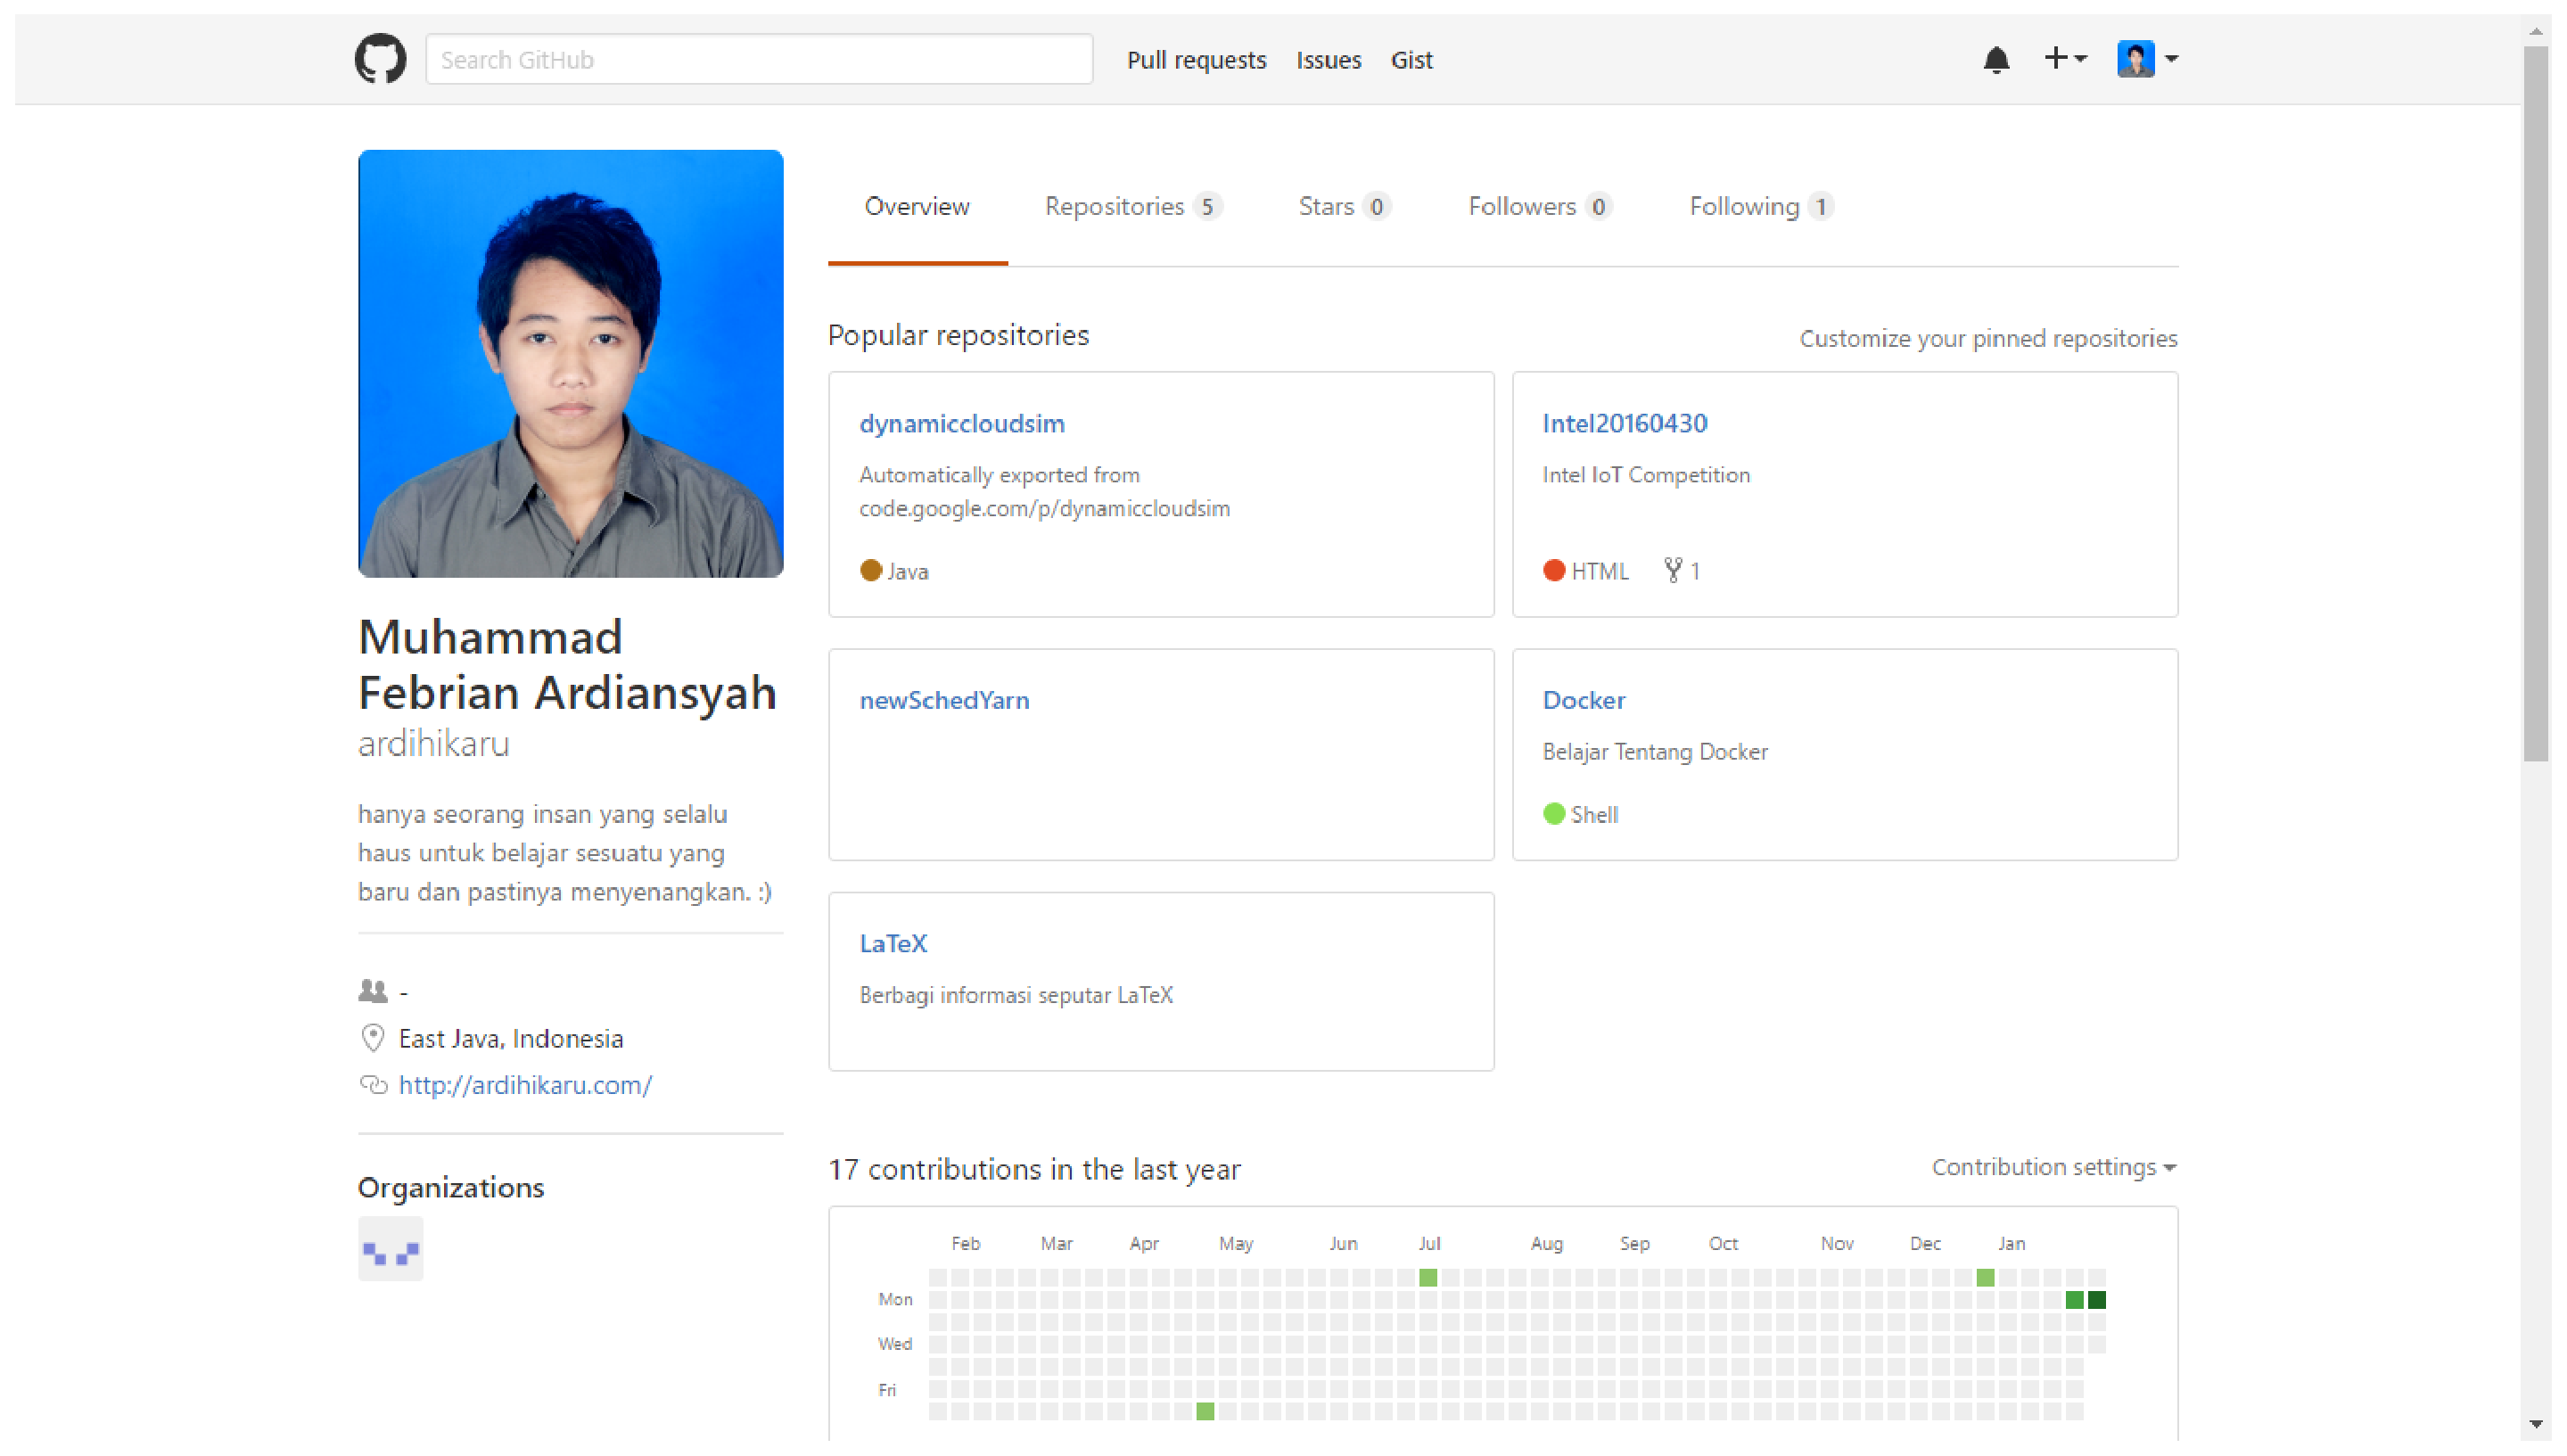
\includegraphics[width=\textwidth, keepaspectratio]{github}
%       \caption{Food choosing}
%       \label{fig:fig1a}
%   \end{subfigure}
%   \begin{subfigure}[b]{0.48\textwidth}
%       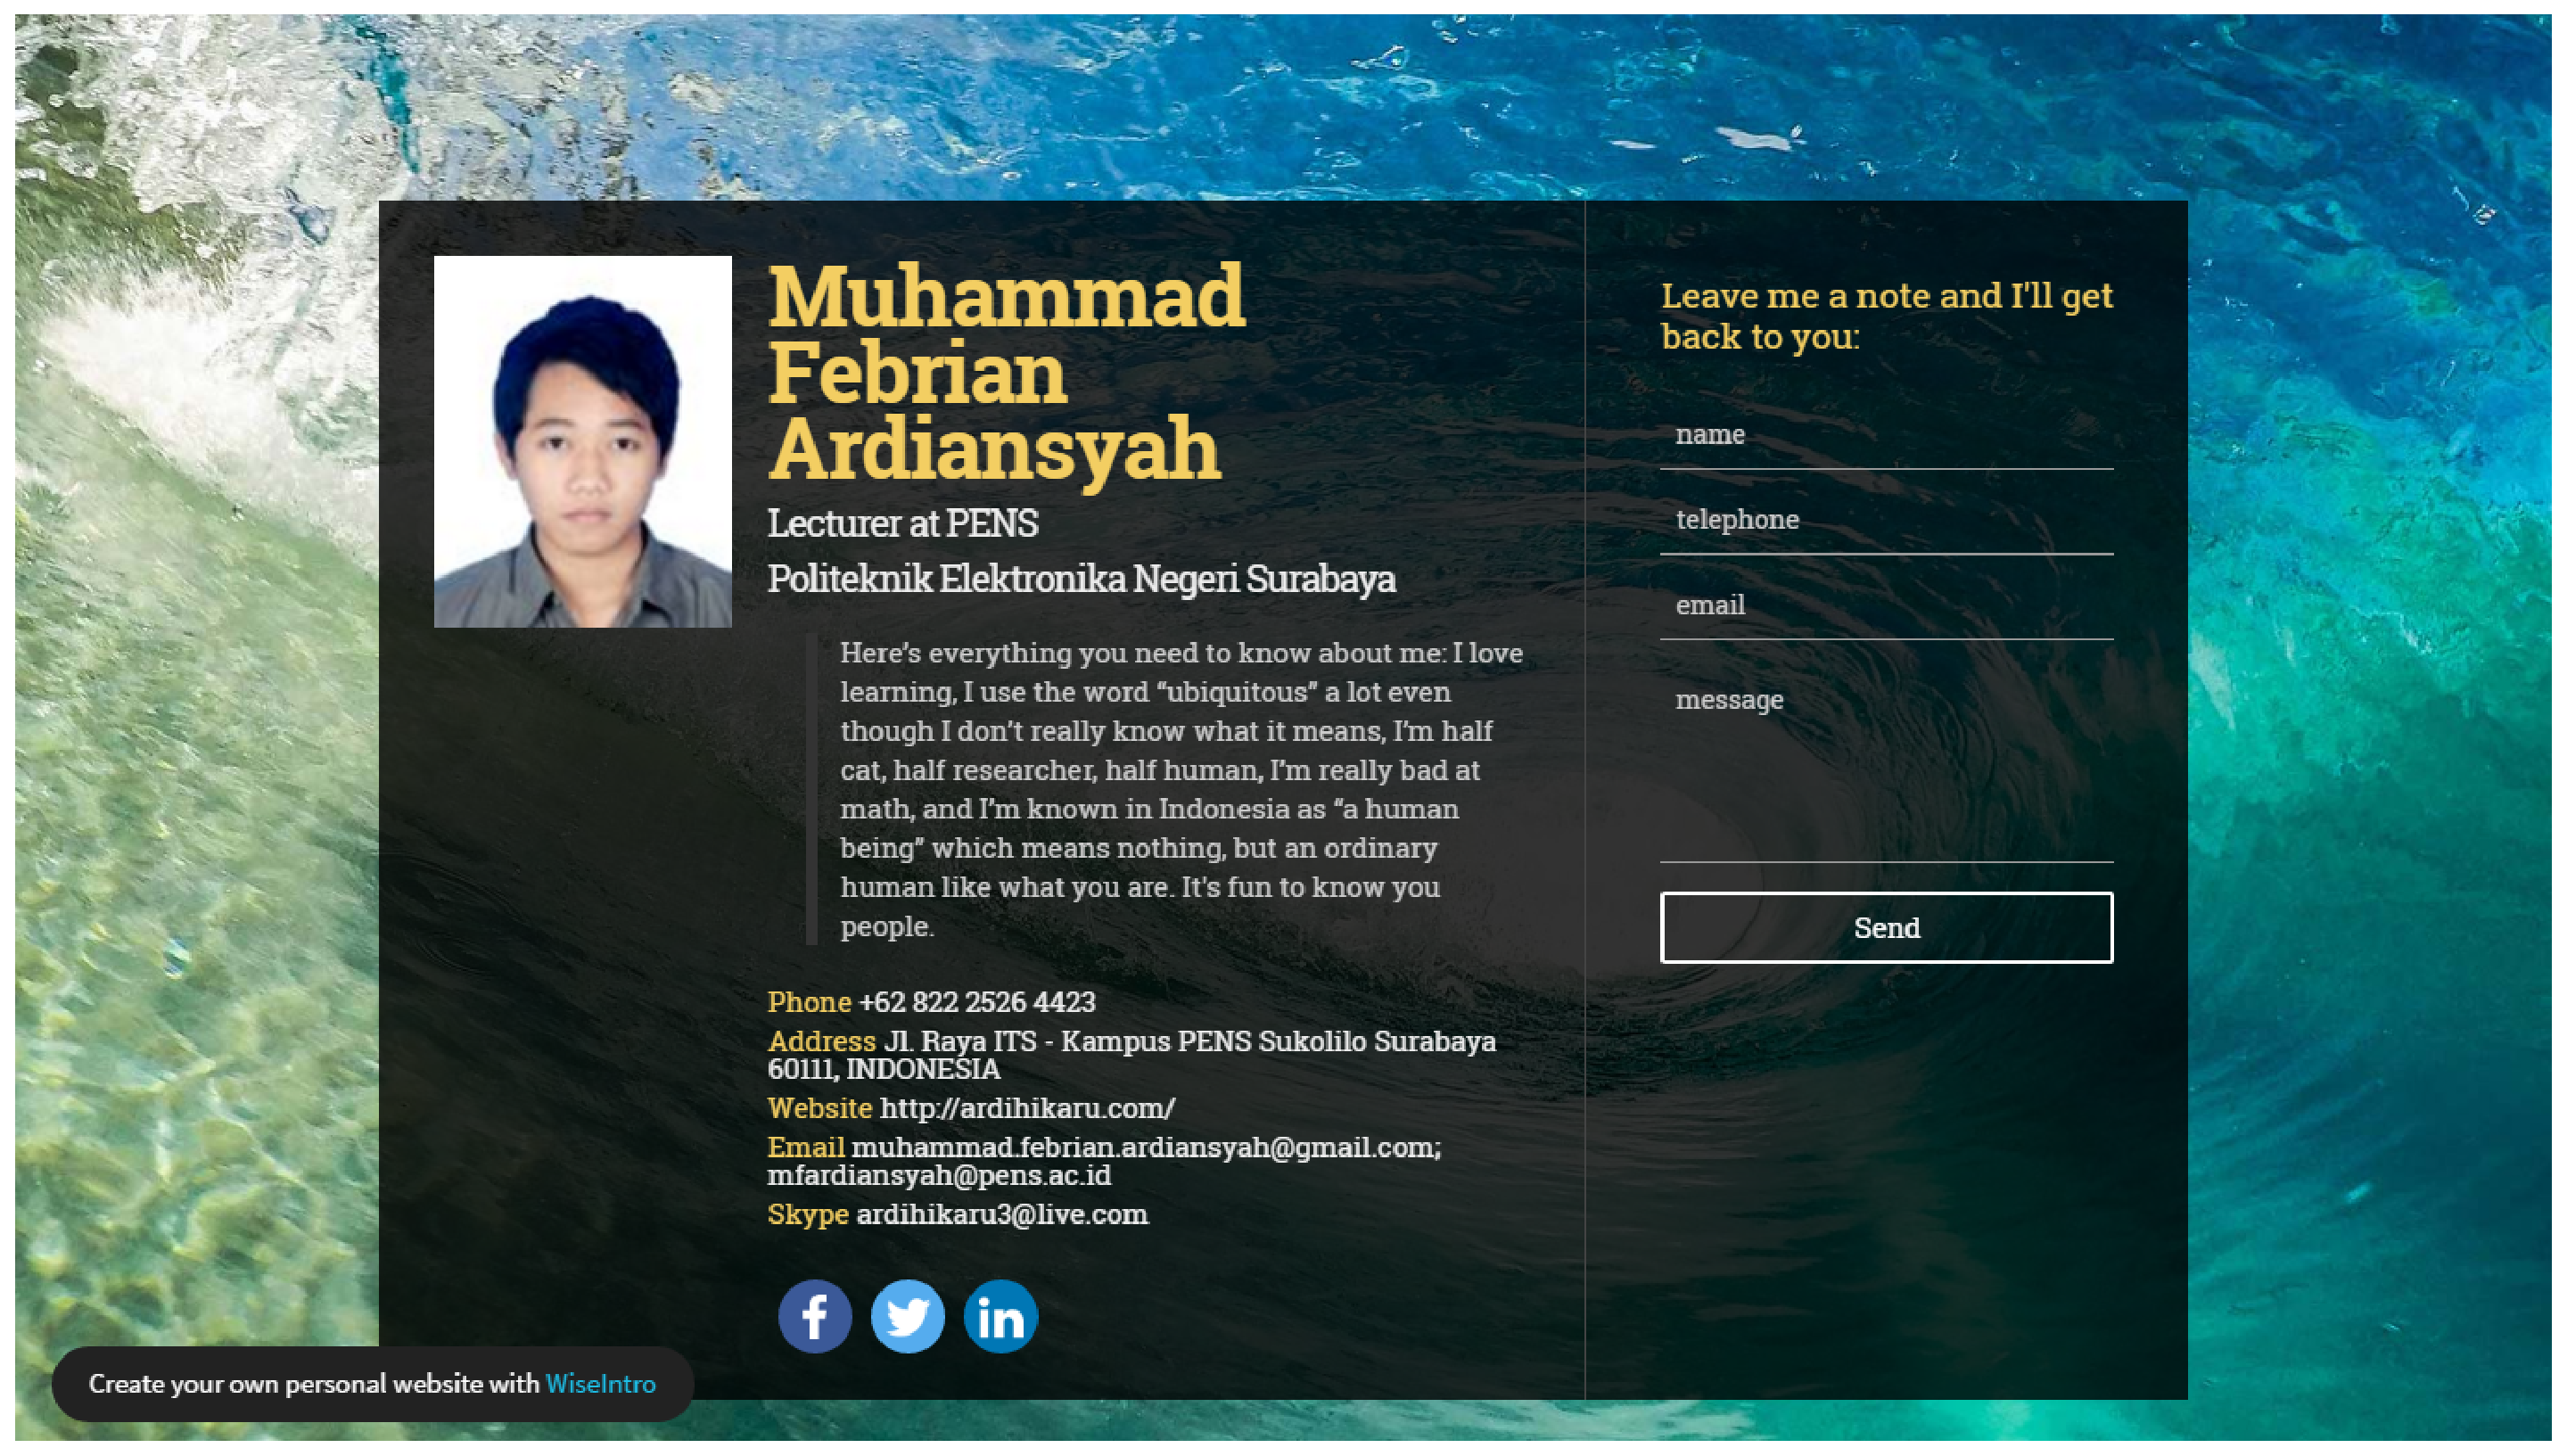
\includegraphics[width=\textwidth, keepaspectratio]{intro}
%       \caption{Interrelationship of different factors for different consumers}
%       \label{fig:fig1b}
%   \end{subfigure}
%   \caption{The difficulties of choosing food and its different adverse reactions}\label{fig1}
%\end{figure*}
%

\begin{figure}[H]
\centering
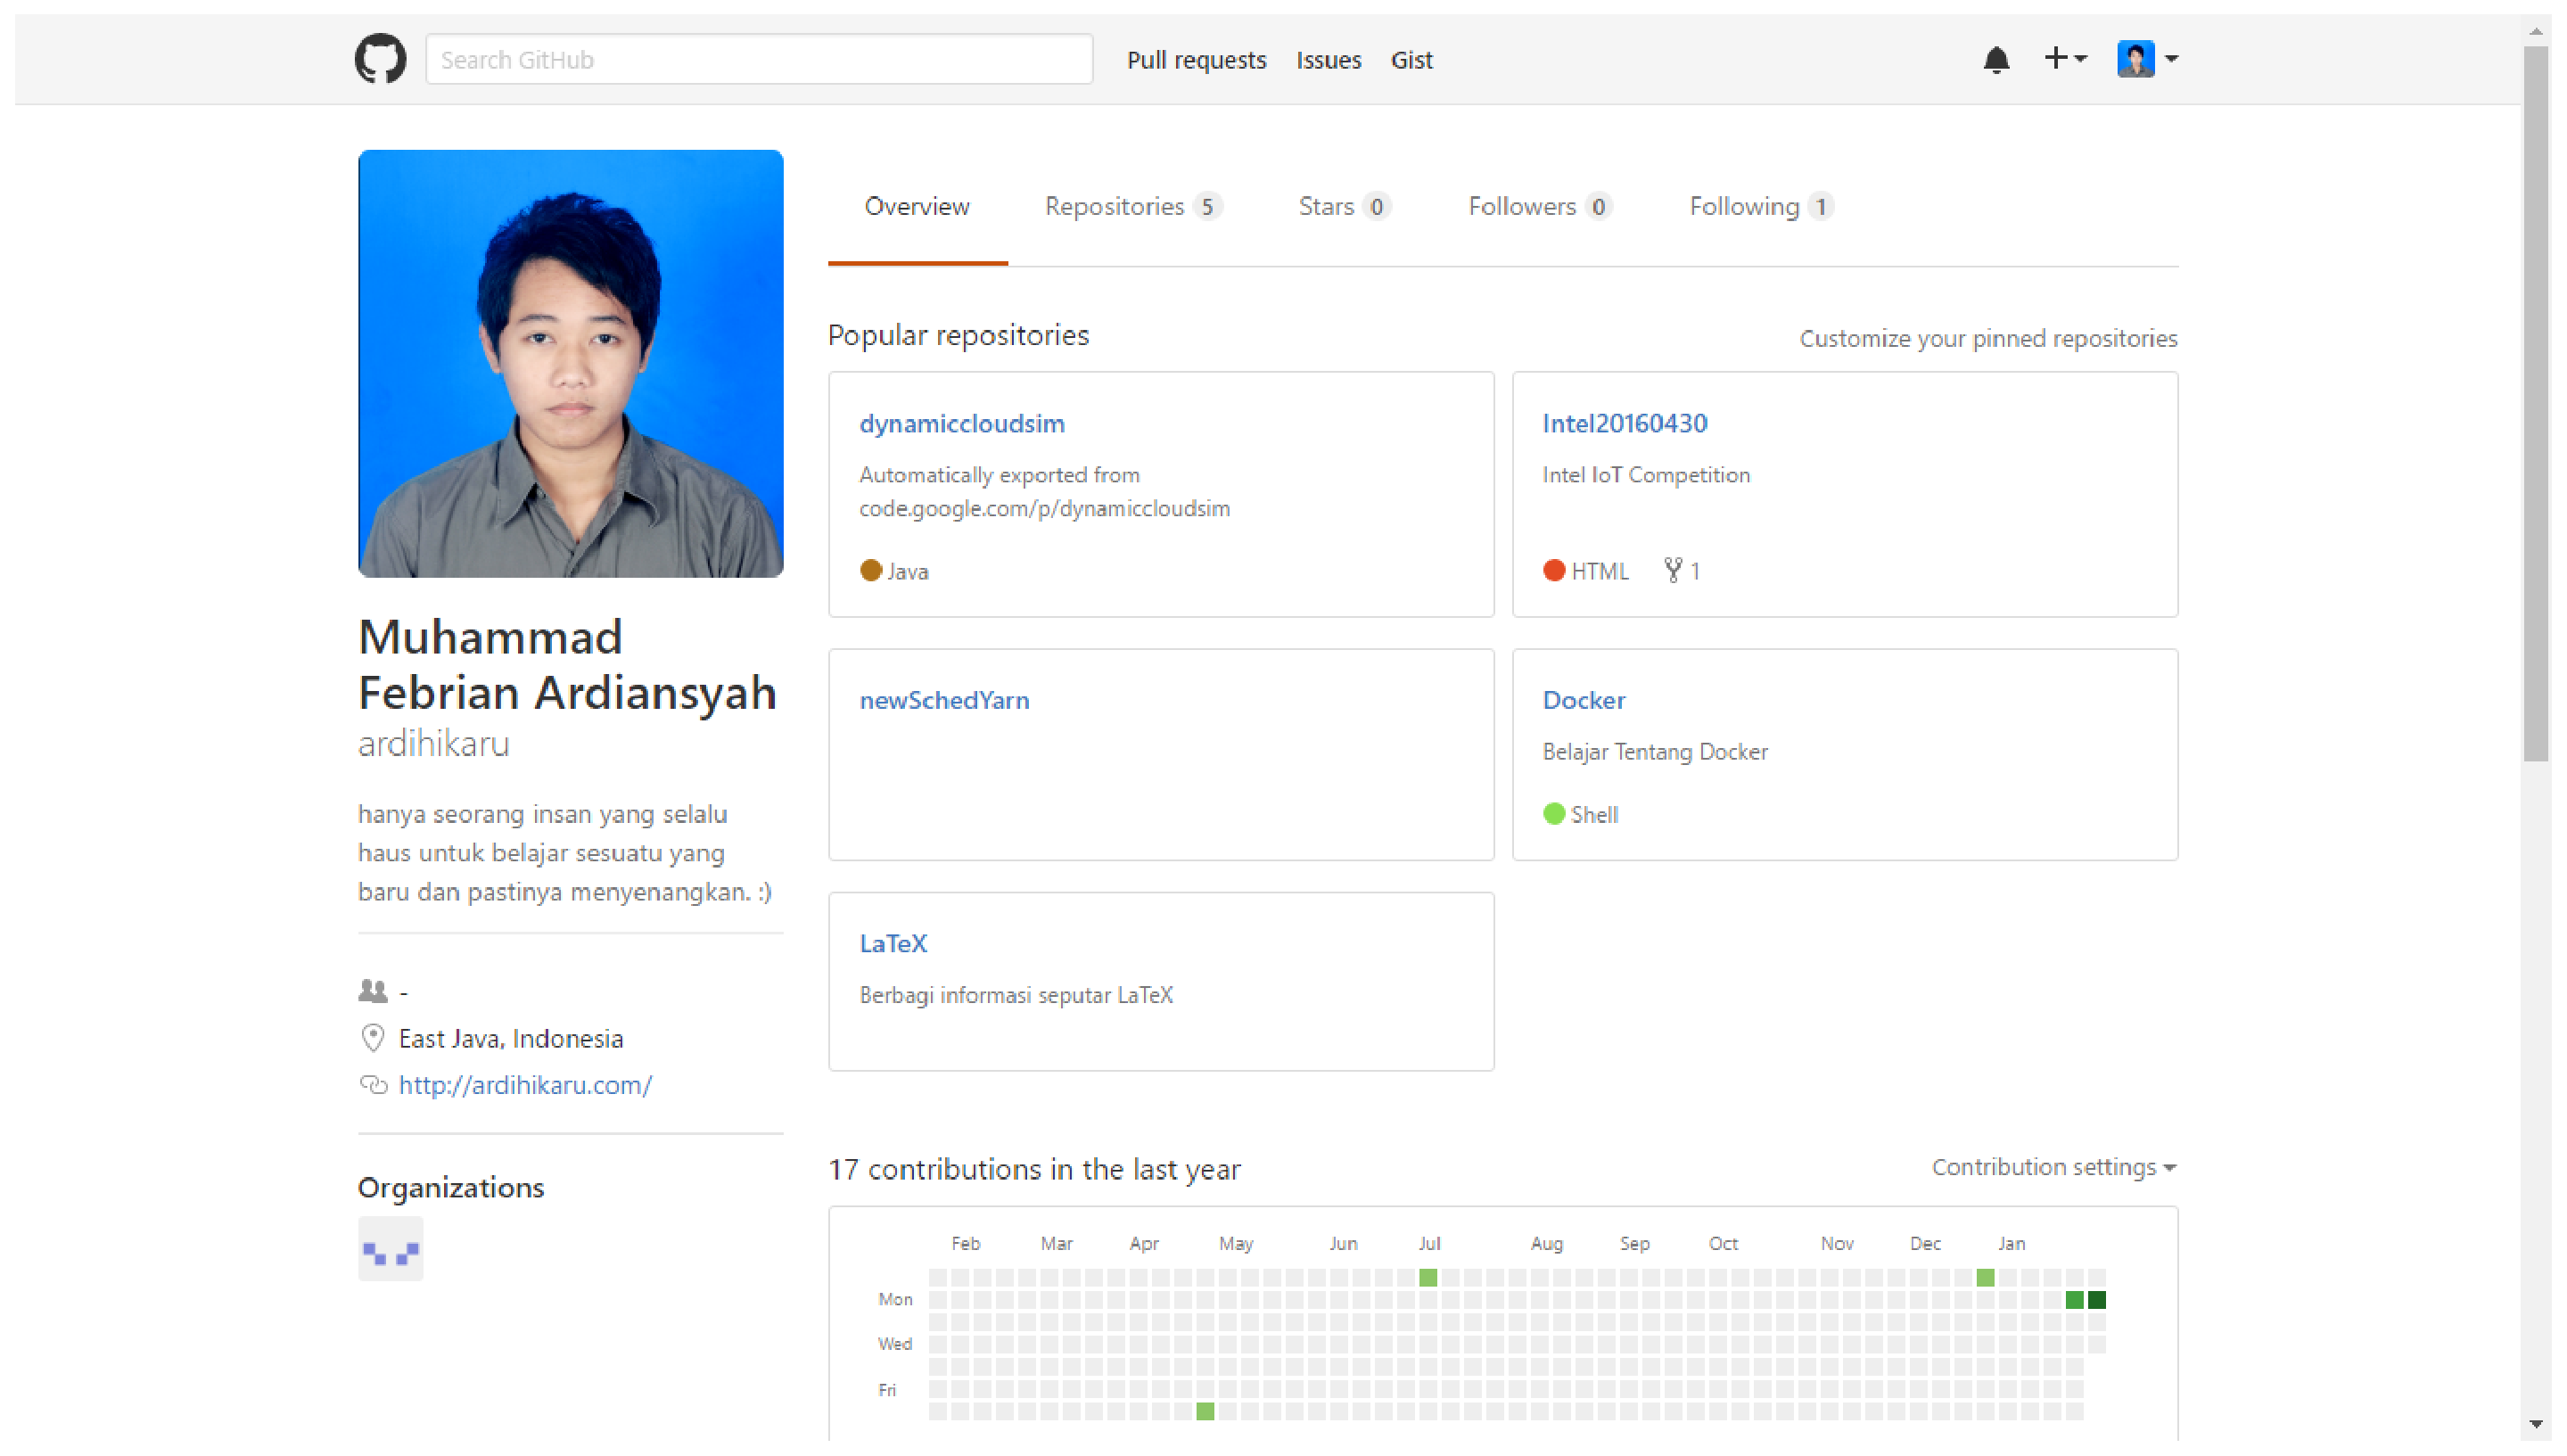
\includegraphics[width=120mm, height=120mm, keepaspectratio]{github}
\caption{Intro}
\label{fig:fig1a}
\end{figure}

\begin{figure}[H]
\centering
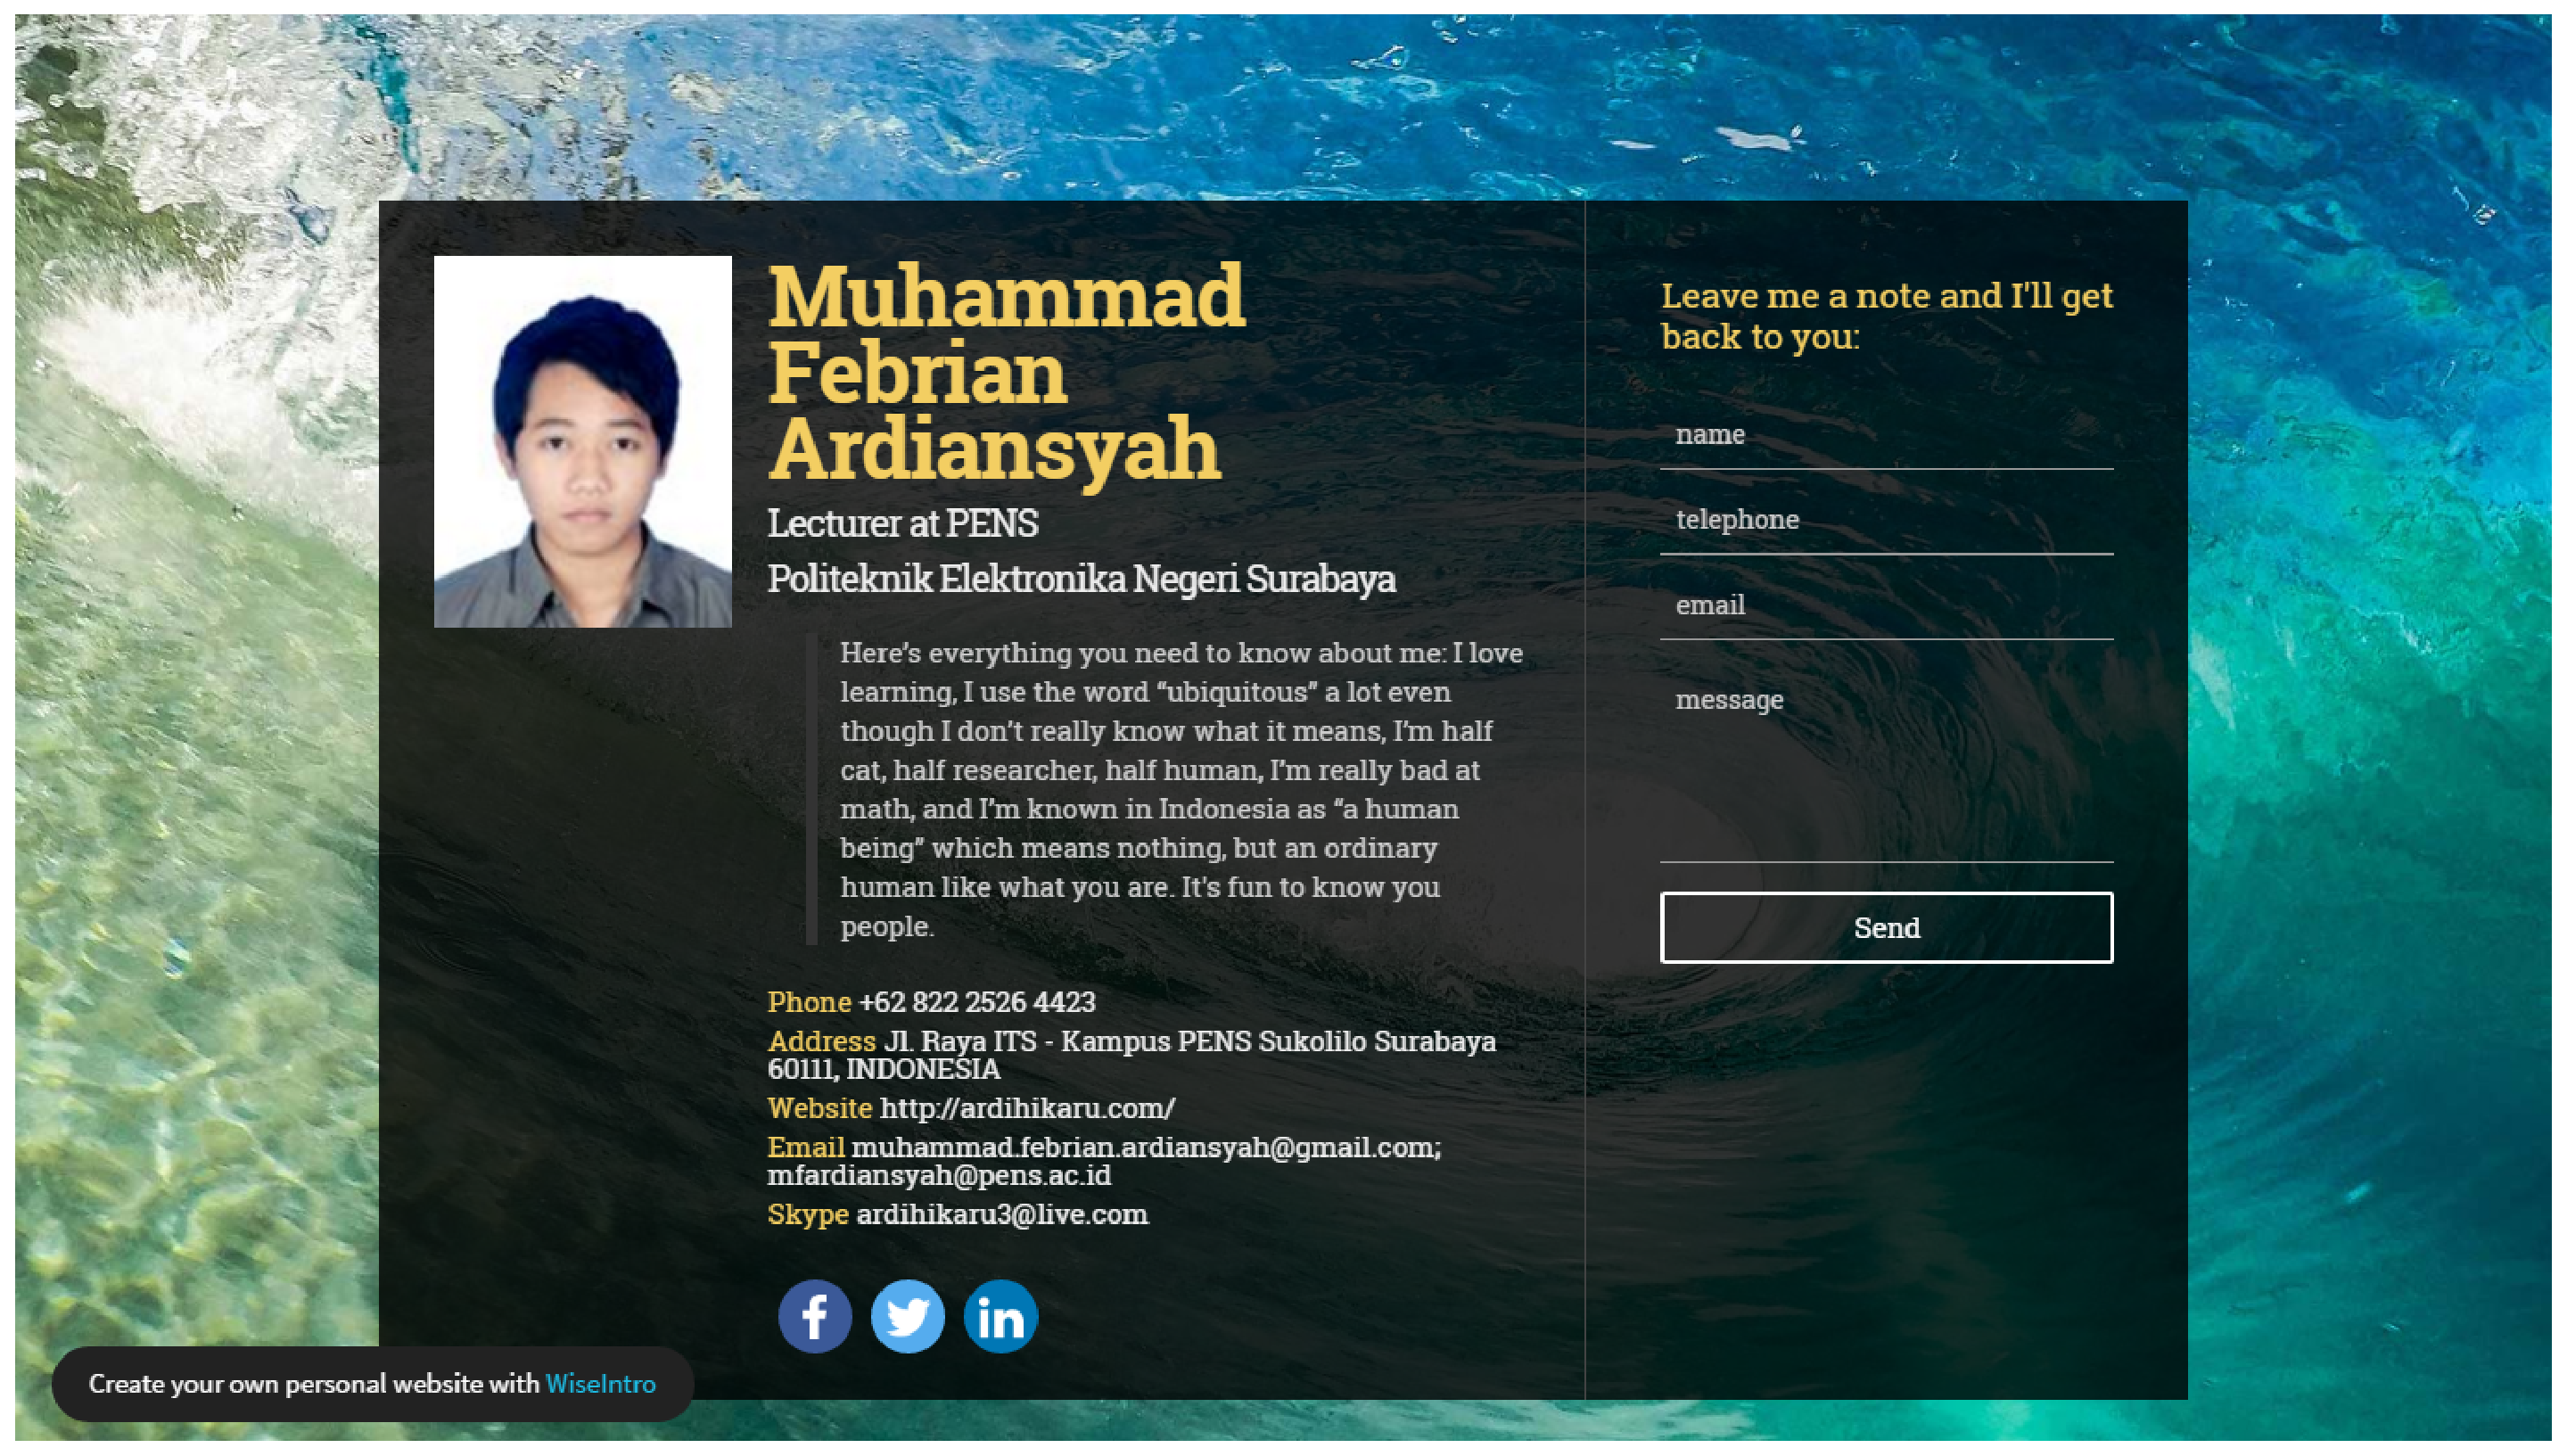
\includegraphics[width=120mm, height=120mm, keepaspectratio]{intro}
\caption{Intro}
\label{fig:fig1b}
\end{figure}

\section{Name of the section 1: e.g. Using figures}
Subsection is here. In latex, it is suggested to use $.eps$ extension as our figure files. Do not ask me why, just trust me, it works! haha. Saran saya, gunakanlah ekstensi $.eps$ untuk gambar-gambar anda. Jangan ditanya ya, percaya saja. (Why? Google it yourself!). 

I use this $online tool$ \footnote{\label{note:eps_converter1}\url{http://www.tlhiv.org/rast2vec/}}. to convert my images into EPS format (resulted smaller and acceptable size). However, sometimes the webpage went offline. If you find some alternative sites, please fell free to share with me, with us.

Use $\backslash ref\{fig:fig1a\}$ (example: Fig.~\ref{fig:fig1a}) to show a figure. In Fig.~\ref{fig:fig1a}, it gives an example of a figure with multiple subfigures. Name $fig:fig1a$ is taken from figure's label. Syntax $\backslash ref\{fig:fig1a\}$ digunakan untuk menampilkan gambar yang sudah di-$attach$ di paper ini. Gambar Fig.~\ref{fig:fig1a} mencontohkan sebuah gambar dengan beberapa sub-gambar.

\begin{figure}[H]
\centering
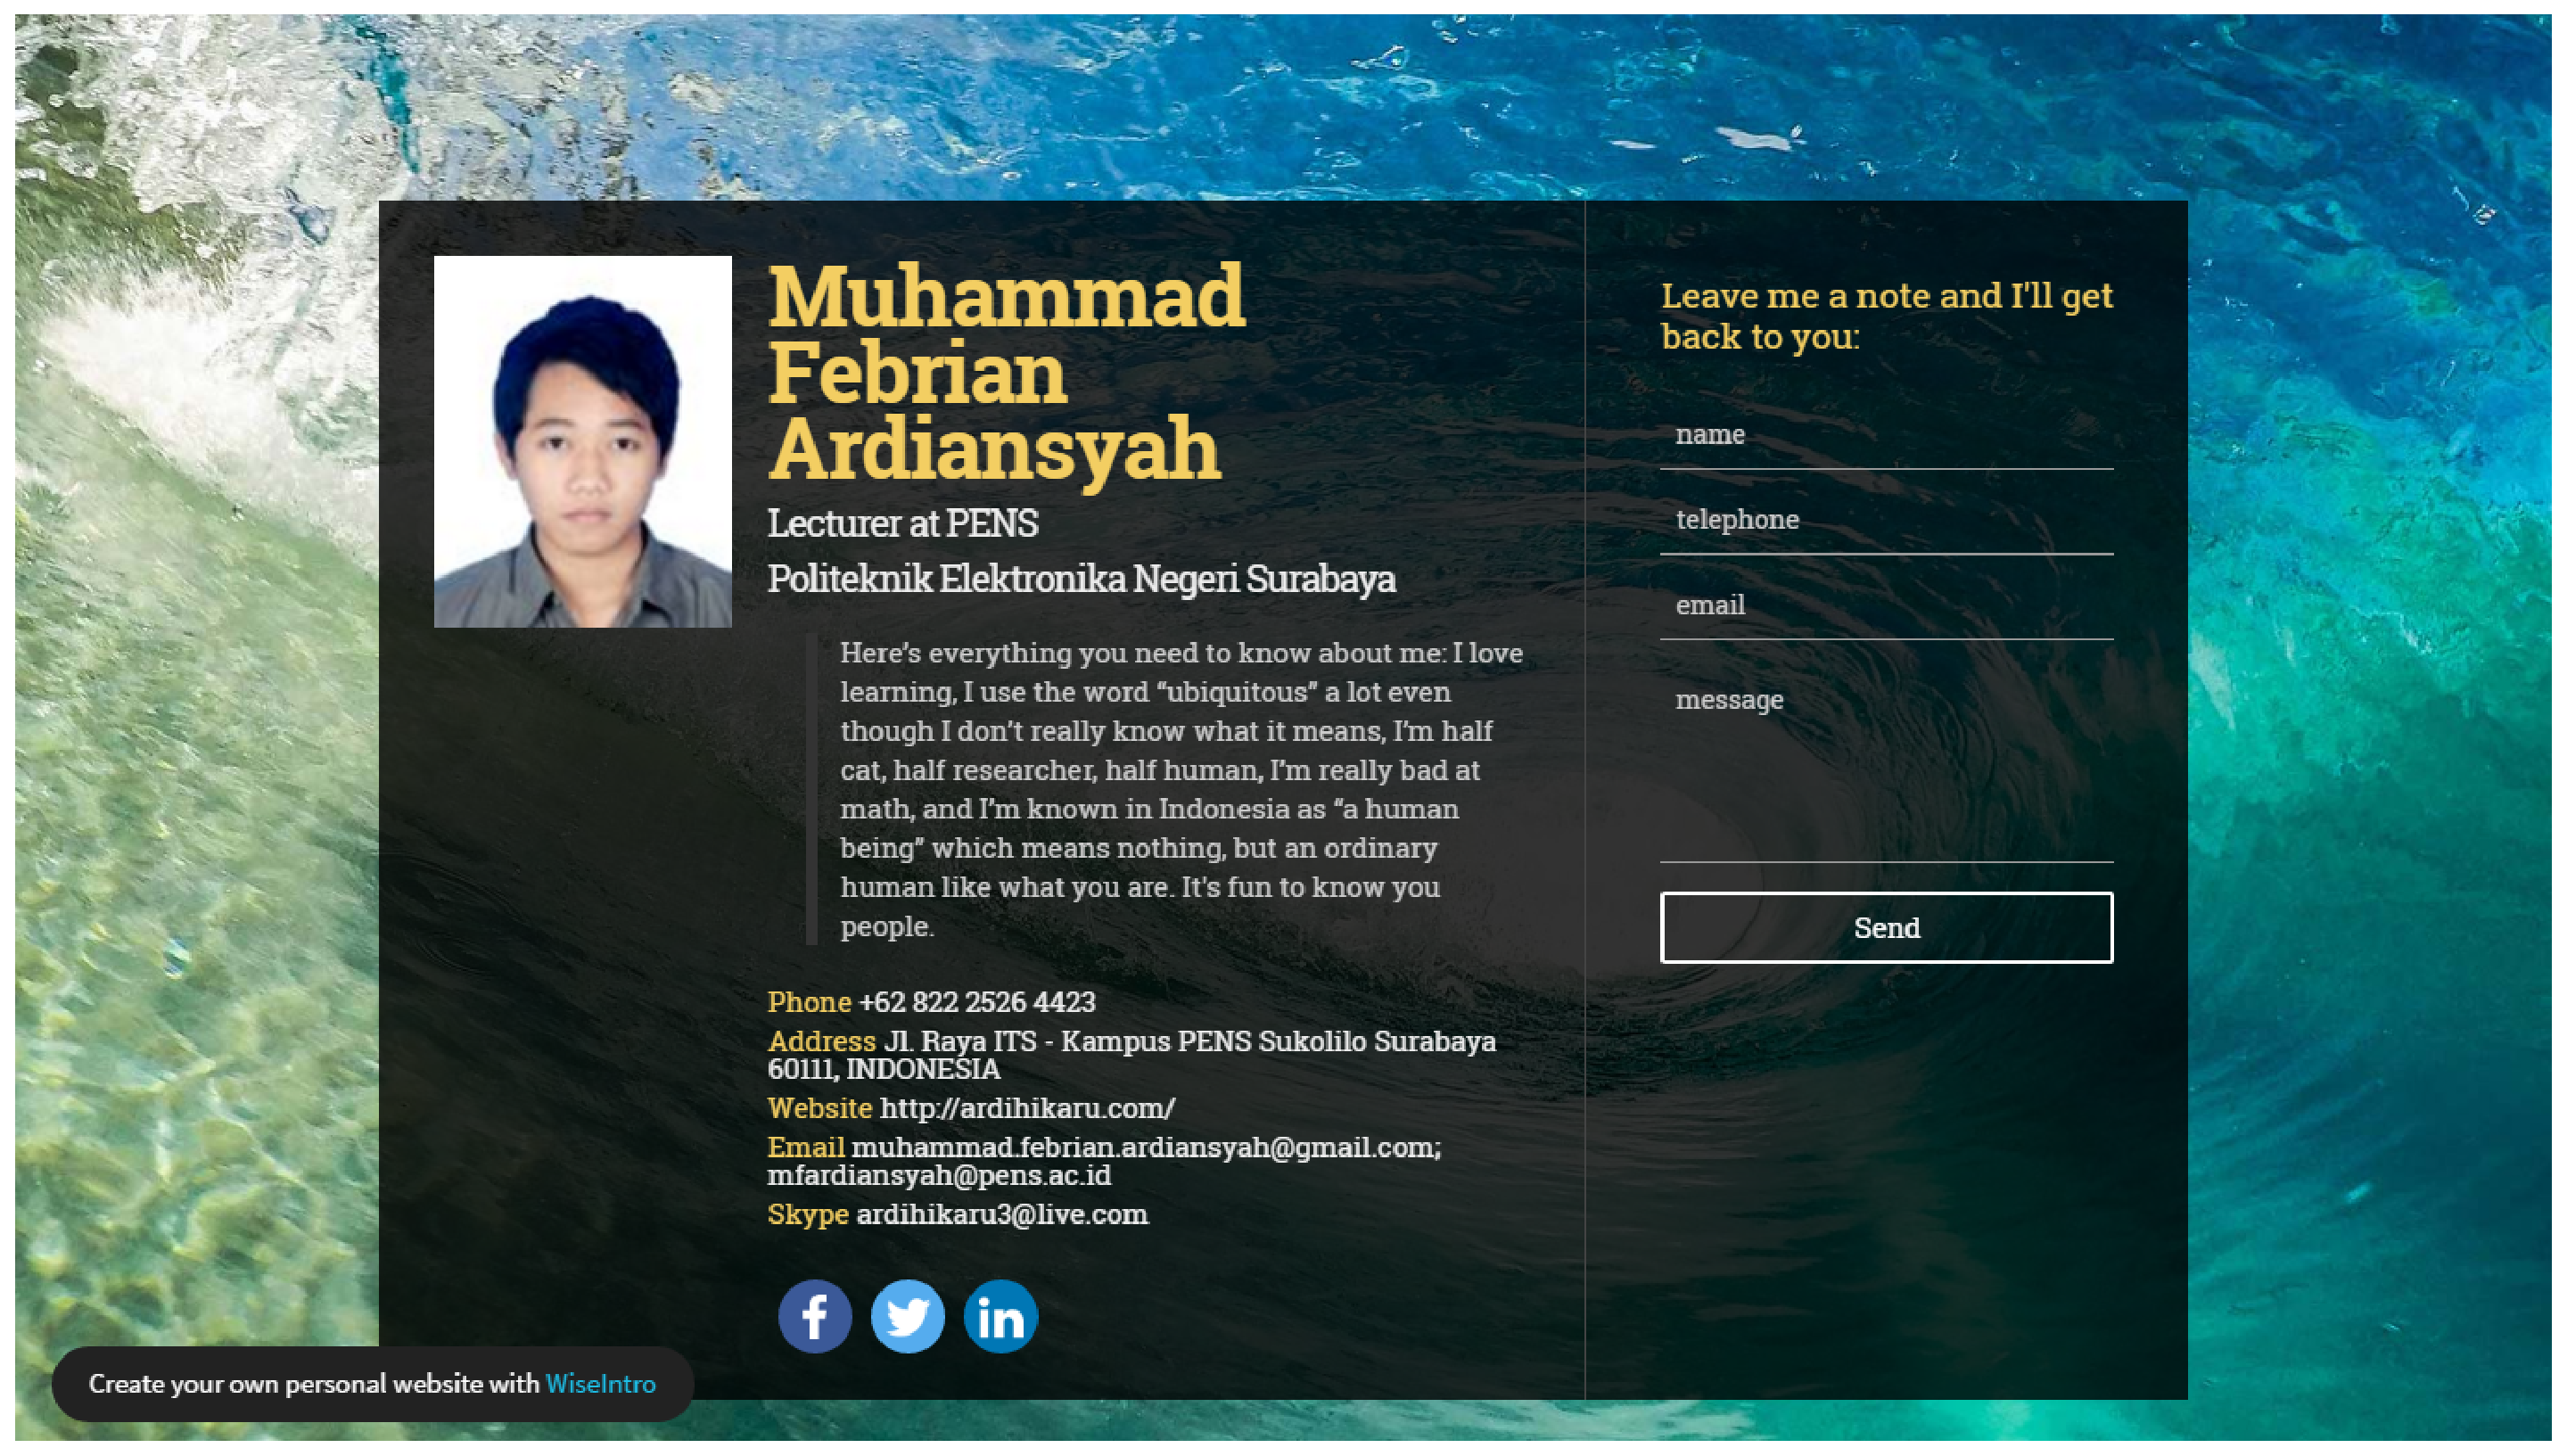
\includegraphics[width=120mm, height=120mm, keepaspectratio]{intro}
\caption{Intro}
\label{fig:fig2}
\end{figure}

Here is another way plot a figure. Fig.~\ref{fig:fig2} is a single figure. There are many ways to plot figures. For the further information, you can check it into $Latex \lq s~wiki$ \footnote{\label{note:latex_wiki_figures}\url{https://en.wikibooks.org/wiki/LaTeX/Floats,_Figures_and_Captions}}. Berikut merupakan cara lain untuk menampilkan gambar. Fig.~\ref{fig:fig2} adalah contoh untuk menampilkan sebuah gambar. Untuk informasi lebih detail, silahkan merujuk $Latex \lq s~wiki$ \footnotemark[\ref{note:latex_wiki_figures}] (yang ini menggunakan rujukan $footnote$). 

Here you may find this itemizing useful.
\begin{itemize}
  \item Item 1.
  \item Item 2.
  \item Item 3.
\end{itemize}

End of introduction section. You may close it with a summary like this: \textquote{\textit{In the rest of this paper, the related works are reviewed in Section 2. Our proposed architecture and system model is discussed in Section 3. Section 4 discusses the methodology we are using our proposed architecture. Then, Section 5 evaluates our research study with some simulation results. Finally, Section 6 summarizes this paper}}. Lanjuutttt...


 % Intro, motivation, goal, contrib., problem formulations.
\chapter{Related Work}
\hspace{0.7cm}

\label{chap:rltwrk} 

\section{Recent proposed custom schedulers}
Related works' here. Tuliskan related work disini.
 % related work
\chapter{Proposed Protocols}

\label{chap:propprotocol} 

\section{System Model}
Content goes here... 

\subsection{Just Another Subsection} 
Let's discuss about $equation$.


\subsubsection{Just Another subsub: Equation example}
Example 1: BMI Formula \cite{nameofref1}. Syntax $\backslash ref\{eq:1\}$ (Example: \ref{eq:1}) is used to call the equation. Contoh 1: Rumus BMI \cite{nameofref1}. Silahkan gunakan syntax $\backslash ref\{eq:1\}$ (Contoh: \ref{eq:1}) untuk memanggil equation tersebut.

% BMI equation here
\begin{equation}‎
\label{eq:1}
BMI‎ ‎=‎ \frac {we} {he^2}
\end{equation}‎

In equation \ref{eq:2}, it gives another example of how to make use of this $equation$ syntax. Di equation \ref{eq:2} ditunjukkan bagaimana cara lain dalam penggunaan syntax ini.

\begin{equation}‎
\label{eq:2}
K(U, W, C) = 
\mathlarger{\mathlarger{‎‎\sum}}_{i=1}^{N‎}
\mathlarger{\mathlarger{‎‎\sum}}_{k=1}^{K}
\gamma_{ik} (\omega_\alpha \times \omega_\beta)_{x_i} D(x_i,c_k)
\end{equation}‎

For further usage, this $reference$ \footnote{\label{note:latex_wiki_math}\url{https://en.wikibooks.org/wiki/LaTeX/Mathematics}} or $this~one$ \footnote{\label{note:latex_wiki_advmath}\url{https://en.wikibooks.org/wiki/LaTeX/Advanced_Mathematics}} might help you. Untuk informasi lebih detail tentang $equation$, silahkan merujuk ke $sini$ \footnotemark[\ref{note:latex_wiki_math}] atau ke $sana$ \footnotemark[\ref{note:latex_wiki_advmath}].

\subsubsection{Just Another subsub: Algorithm example}
Let's go through how do we write an algorithm and how to $summon$ it into our masterpiece! Berikut merupakan cara penulisan algoritma dan pemanggilannya.


\begin{algorithm}[H]
  \caption{Name of the algorithm, contoh: Algojlo untuk pengguna $U$}
  \label{alg:1}
  \begin{algorithmic}[1]
    
		\Require
      \Statex Data Matrik (A, B) $a \times b \to \phi \times y$.
      \Statex Titik datanya $pn = \{p_1, xp_2, ..., p_l\}$; 
      			$~p_i \to namafunc(x,y) = xxx \times yyy$\
      \Statex Set $G$ untuk percobaan.
      
    \Ensure
      \Statex (Pastikan) setiap var $p_i$ berjodoh (ehem) dengan $gueh$.
	
		\Statex
			
		\State Bangkitkan var $P$ acak acak acakkkkk;
			\For  {$i=1$ to $g$} 
				\For  {$k=1$ to $r$} 
					\State Hitung $Rumus 1$; 
					\State Tanya $Rumus 2$; \Comment{(tanya ken, apa?)}
					\State Tinggalkan $Rumus 3$;   
				\EndFor   
			\EndFor 
  \end{algorithmic}
\end{algorithm}

\clearpage

\begin{algorithm}[H]
  \ContinuedFloat
  \caption{Name of the algorithm, contoh: Algojlo untuk pengguna $U$ (continued)}
  \begin{algorithmic}
		
		
			%%%
			\For  {$i=1$ to $g$} 
				\For  {$k=1$ to $r$} 
					\State Hitung $Rumus 1$; 
					\State Tanya $Rumus 2$; \Comment{(tanya ken, apa?)}
					\State Tinggalkan $Rumus 3$;   
				\EndFor   
			\EndFor  
			%%%
			\State Samakan $a = a$;
			\For  {$k=1$ to $D$} 
				\State Makan ${roti}^{isi}_{misis}$; 
				\If {$y_{coba(baru)} \neq g^{dor}$}
					\State Lewati;
			\EndIf
			\EndFor   
			\State Return $y$;
			%%%
			\If {$lanjut(true)$}
				\State Kembali ke $line~6$;
		\EndIf
			
		
  \end{algorithmic}
\end{algorithm}

Penggilan algoritma bisa menggunakan: $\backslash ref\{alg:1\}$, contoh: \ref{alg:1}.

Contoh equation di paragraf: $\alpha_{coba} = \mathlarger{\mathlarger{‎‎\sum}}_{x=1}^{A‎} b^{cd}_e$, bisa juga $\alpha_{min} = MIN(\alpha)$ and $\alpha_{max} = MAX(\alpha)$. Gunakan $\{<<code here..>>\}$ jika variabel berupa kata.

\subsubsection{Just Another subsub: Table example}
Check it out!

\begin{table}[H]
\centering

\begin{tabular}{ |l|r|c| }
\hline
%\multicolumn{3}{ |c| }{Simulation Parameters} \\
%\hline

{Colomn 1} & \multicolumn{2}{ |c| }{Colomn 2 - multi-comlomn} \\ 
\hline %header

\multirow{3}{*}{Var 1 (3)} & 1.000 & \multirow{3}{*}{Detil var 1} \\
 & 2.000 & \\
 & 3.000 & \\ \hline
 
{Var 2} & 10 & {Type of Food} \\ \hline
 
\multirow{5}{*}{Var 3 (5)} & 2 & \multirow{5}{*}{Detil var 2} \\
 & 2 & \\
 & 4 & \\
 & 6 & \\
 & 8 & \\ \hline
 
\multirow{3}{*}{Var 4 (3)} & 10 & \multirow{3}{*}{Detil var 3} \\
 & 20 & \\
 & 30 & \\ \hline
 
\hline
\end{tabular}

\caption{Contoh tabel}
\label{table:example}
\end{table}

Penggilan tabel bisa menggunakan: $\backslash ref\{table:example\}$, contoh: \ref{table:example}.

\subsubsection{Just Another subsub: How to find reference}
You can try using $google scholar$ \footnote{\label{note:google_scholar}\url{https://scholar.google.co.id/}} to get the bib script. Follow this step-by-step from Figures \ref{fig:fig3_1}, \ref{fig:fig3_2}, \ref{fig:fig3_3}, \ref{fig:fig3_4} below.

\begin{figure}[H]
\centering
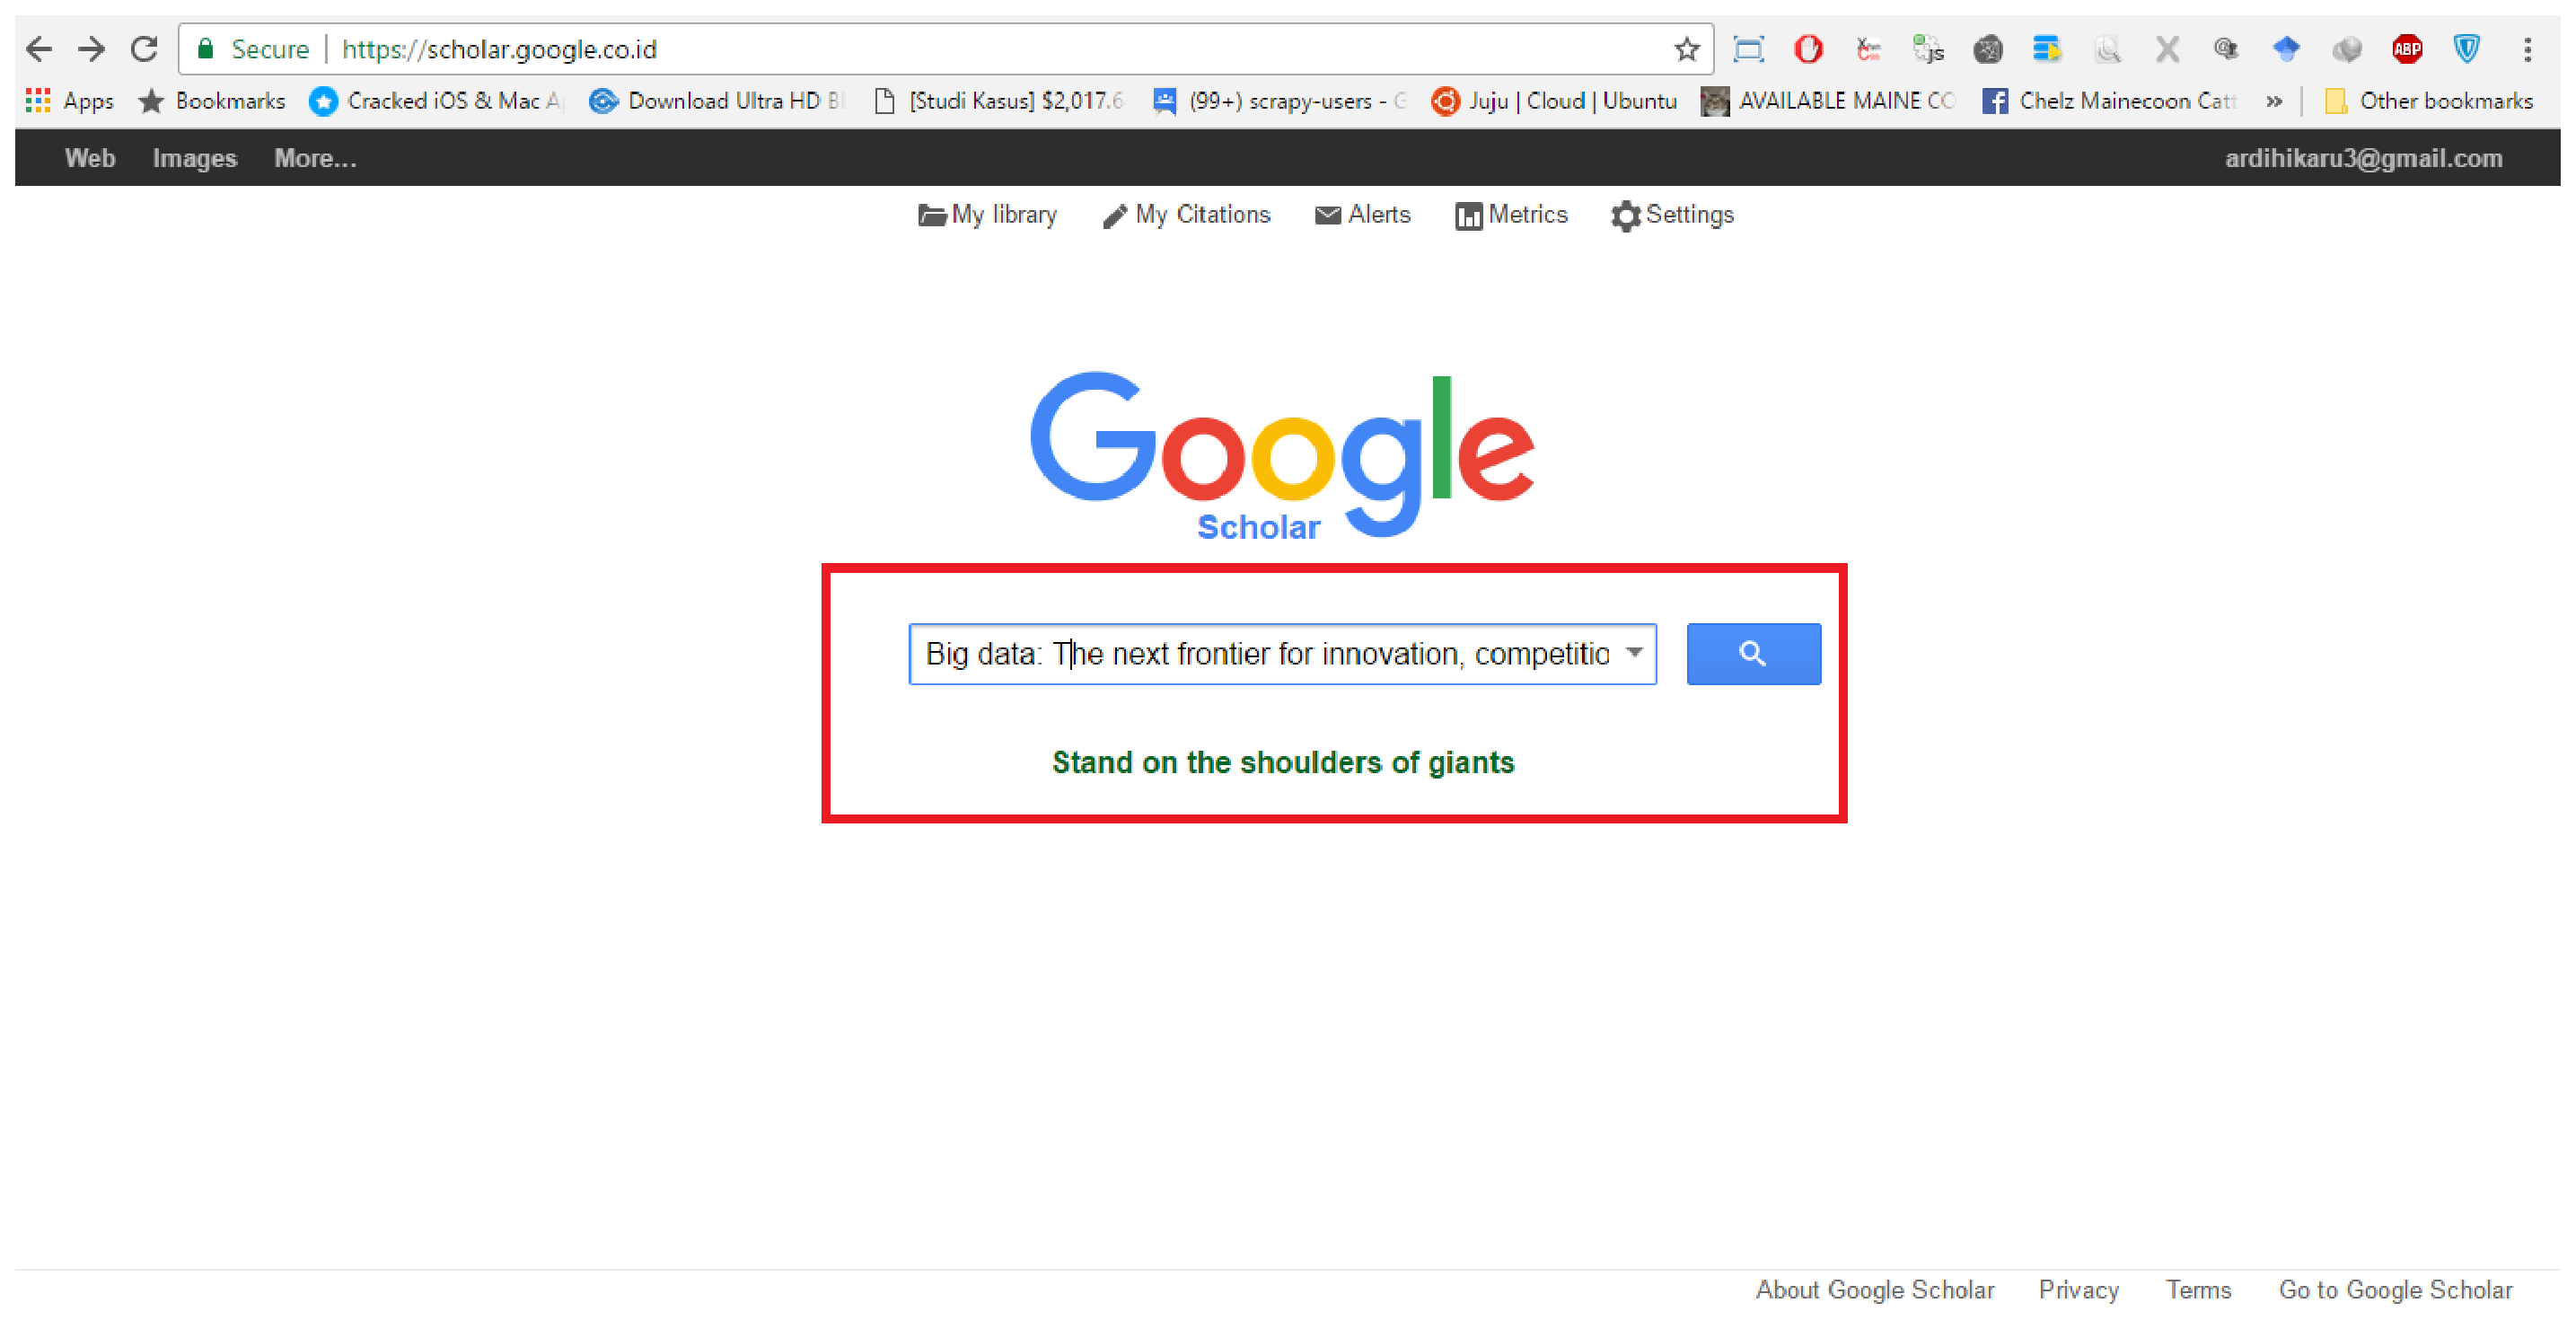
\includegraphics[width=120mm, height=120mm, keepaspectratio]{get_bib_script_part_1}
\caption{Buka Google Scholar}
\label{fig:fig3_1}
\end{figure}

\begin{figure}[H]
\centering
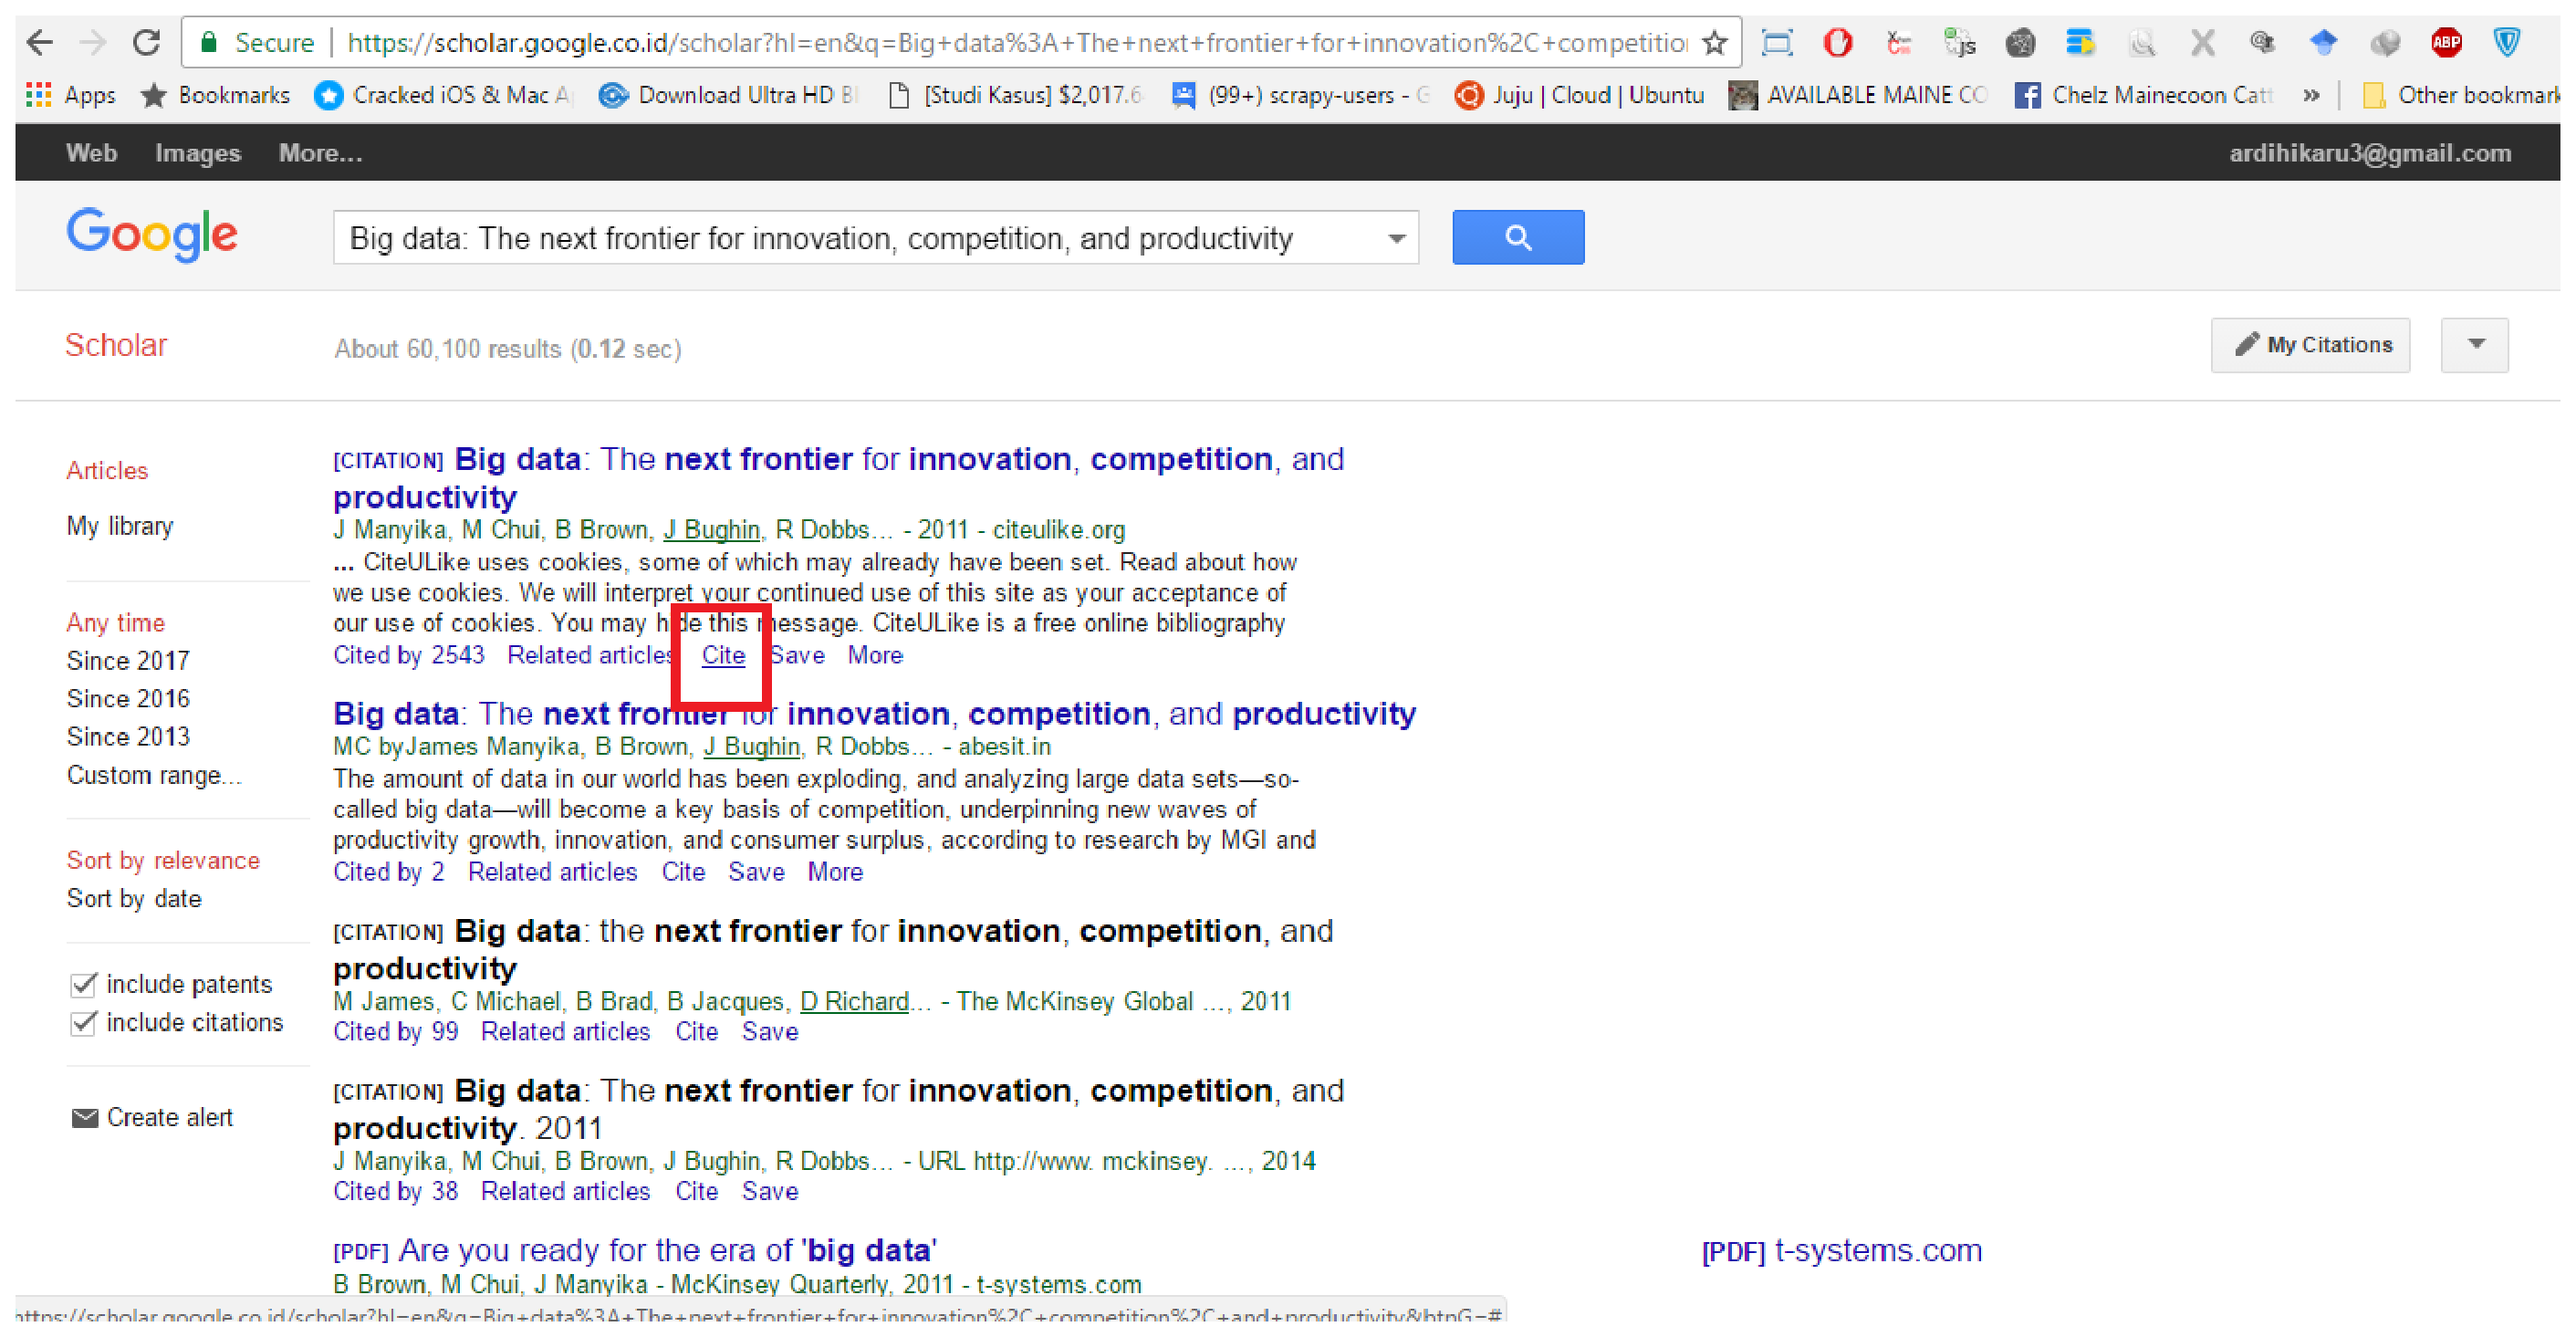
\includegraphics[width=120mm, height=120mm, keepaspectratio]{get_bib_script_part_2}
\caption{Click of the $Cite$ link.}
\label{fig:fig3_2}
\end{figure}

\begin{figure}[H]
\centering
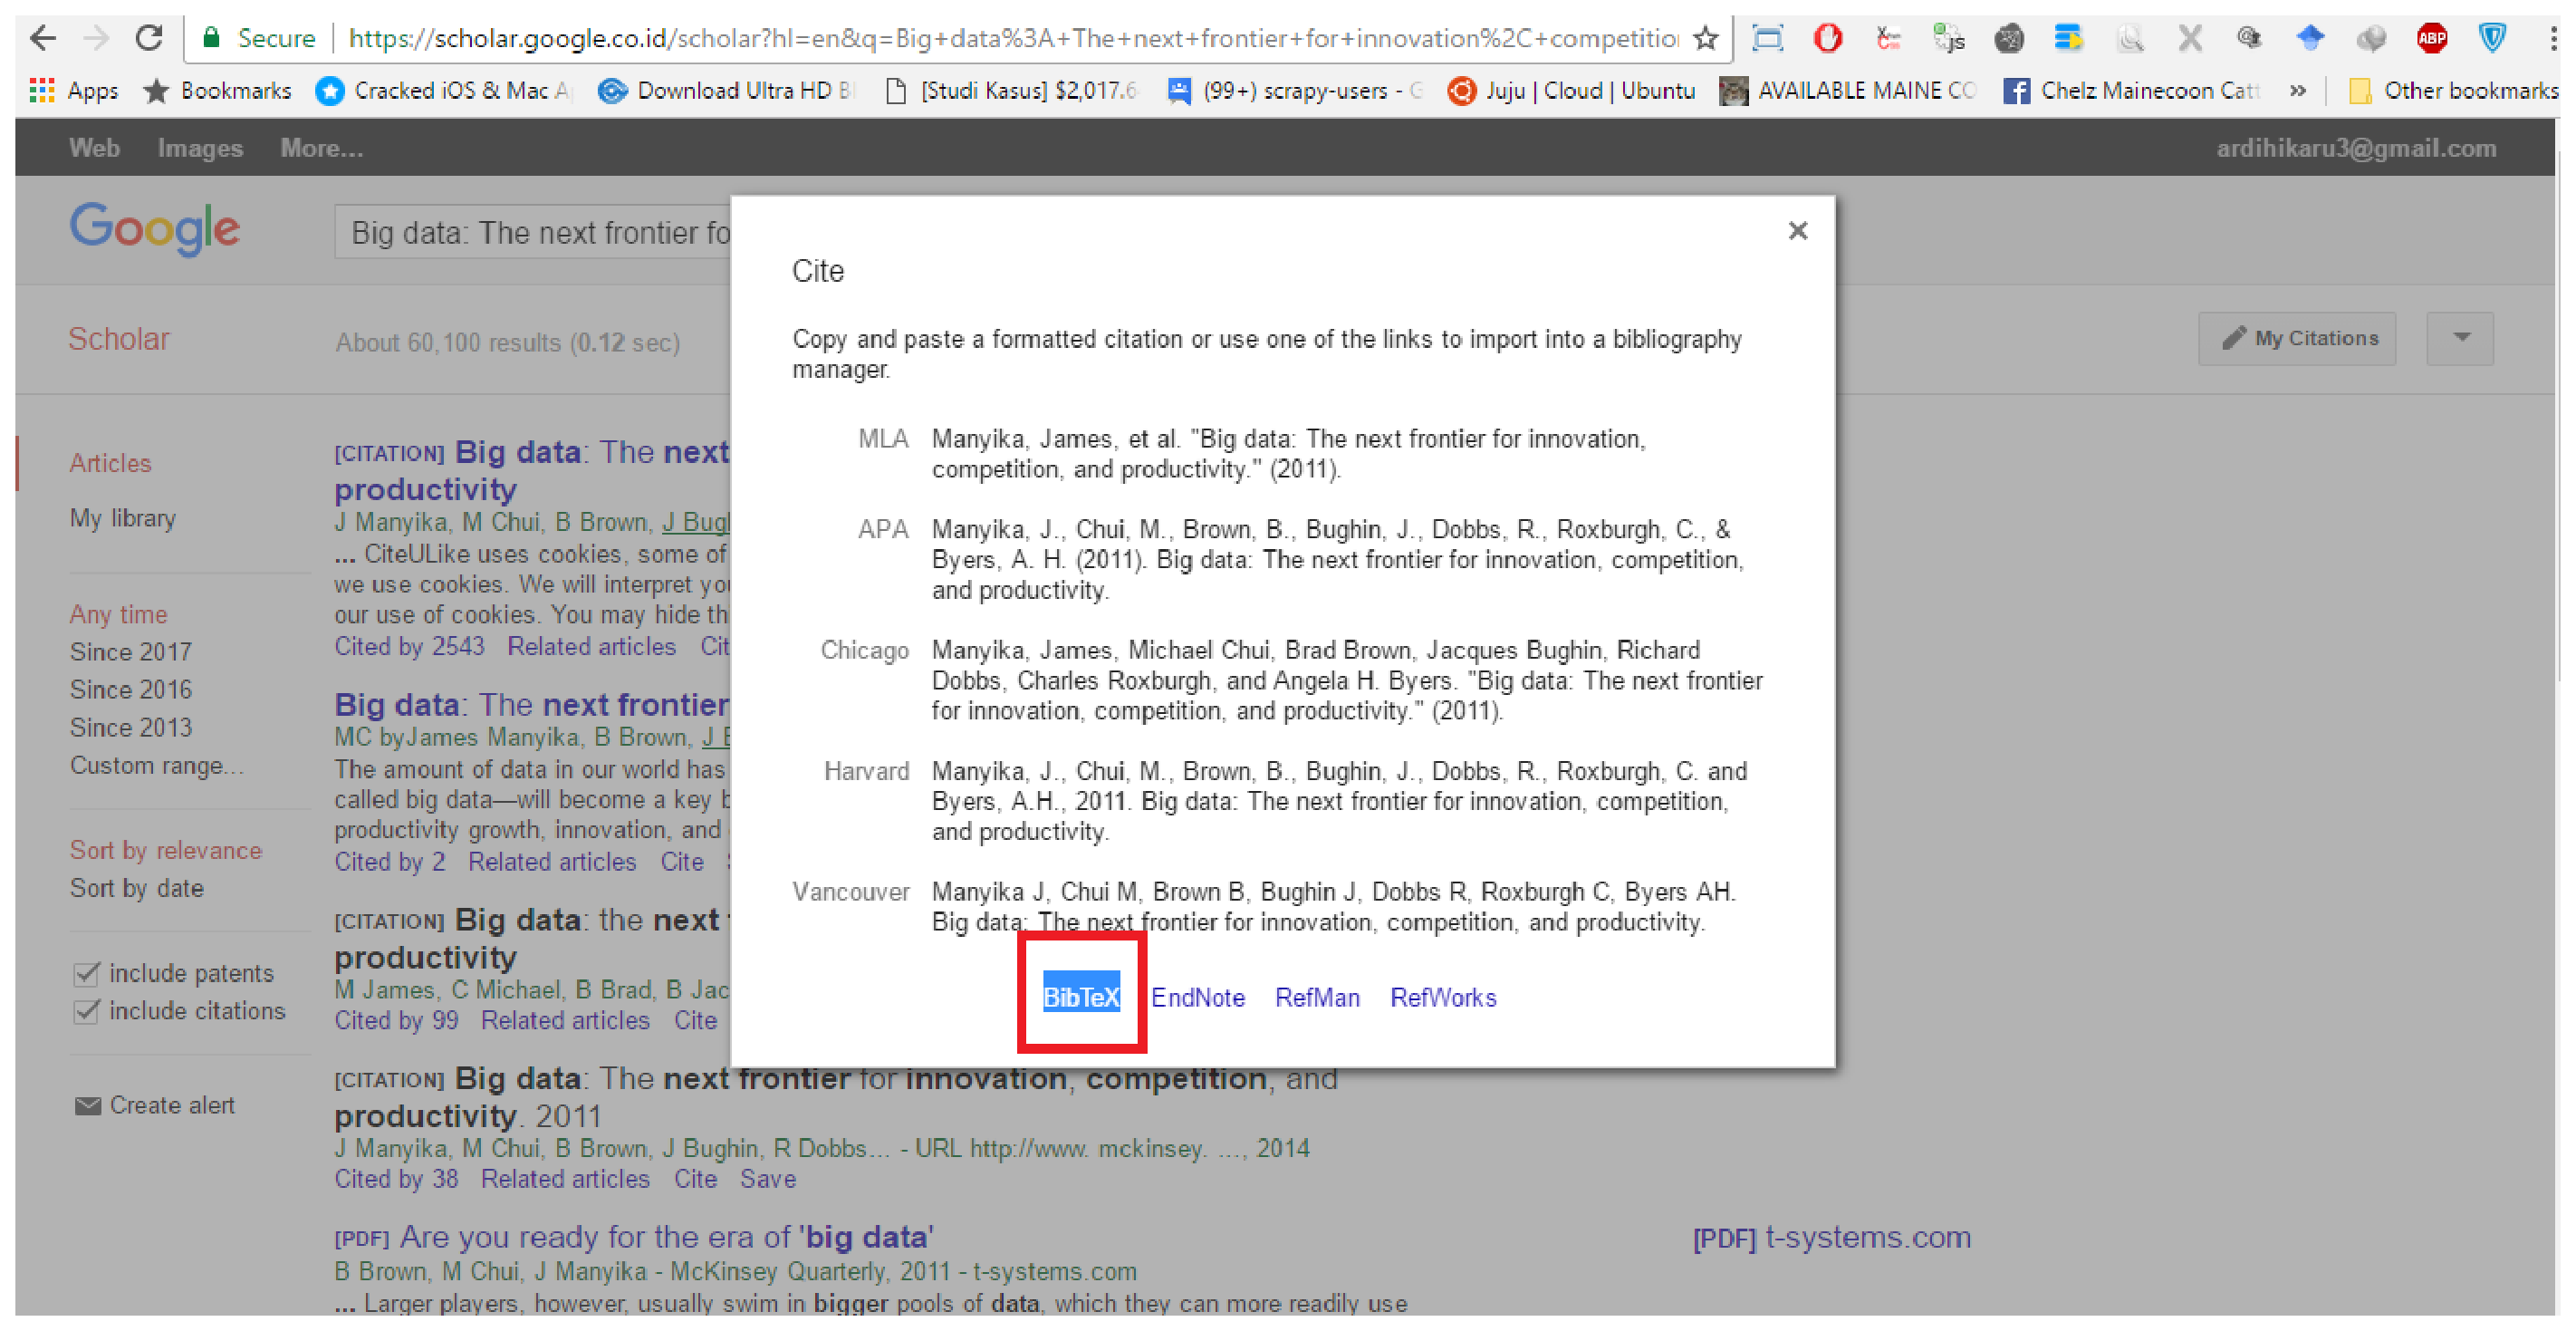
\includegraphics[width=120mm, height=120mm, keepaspectratio]{get_bib_script_part_3}
\caption{Click of the $BibTeX$ link.}
\label{fig:fig3_3}
\end{figure}

\begin{figure}[H]
\centering
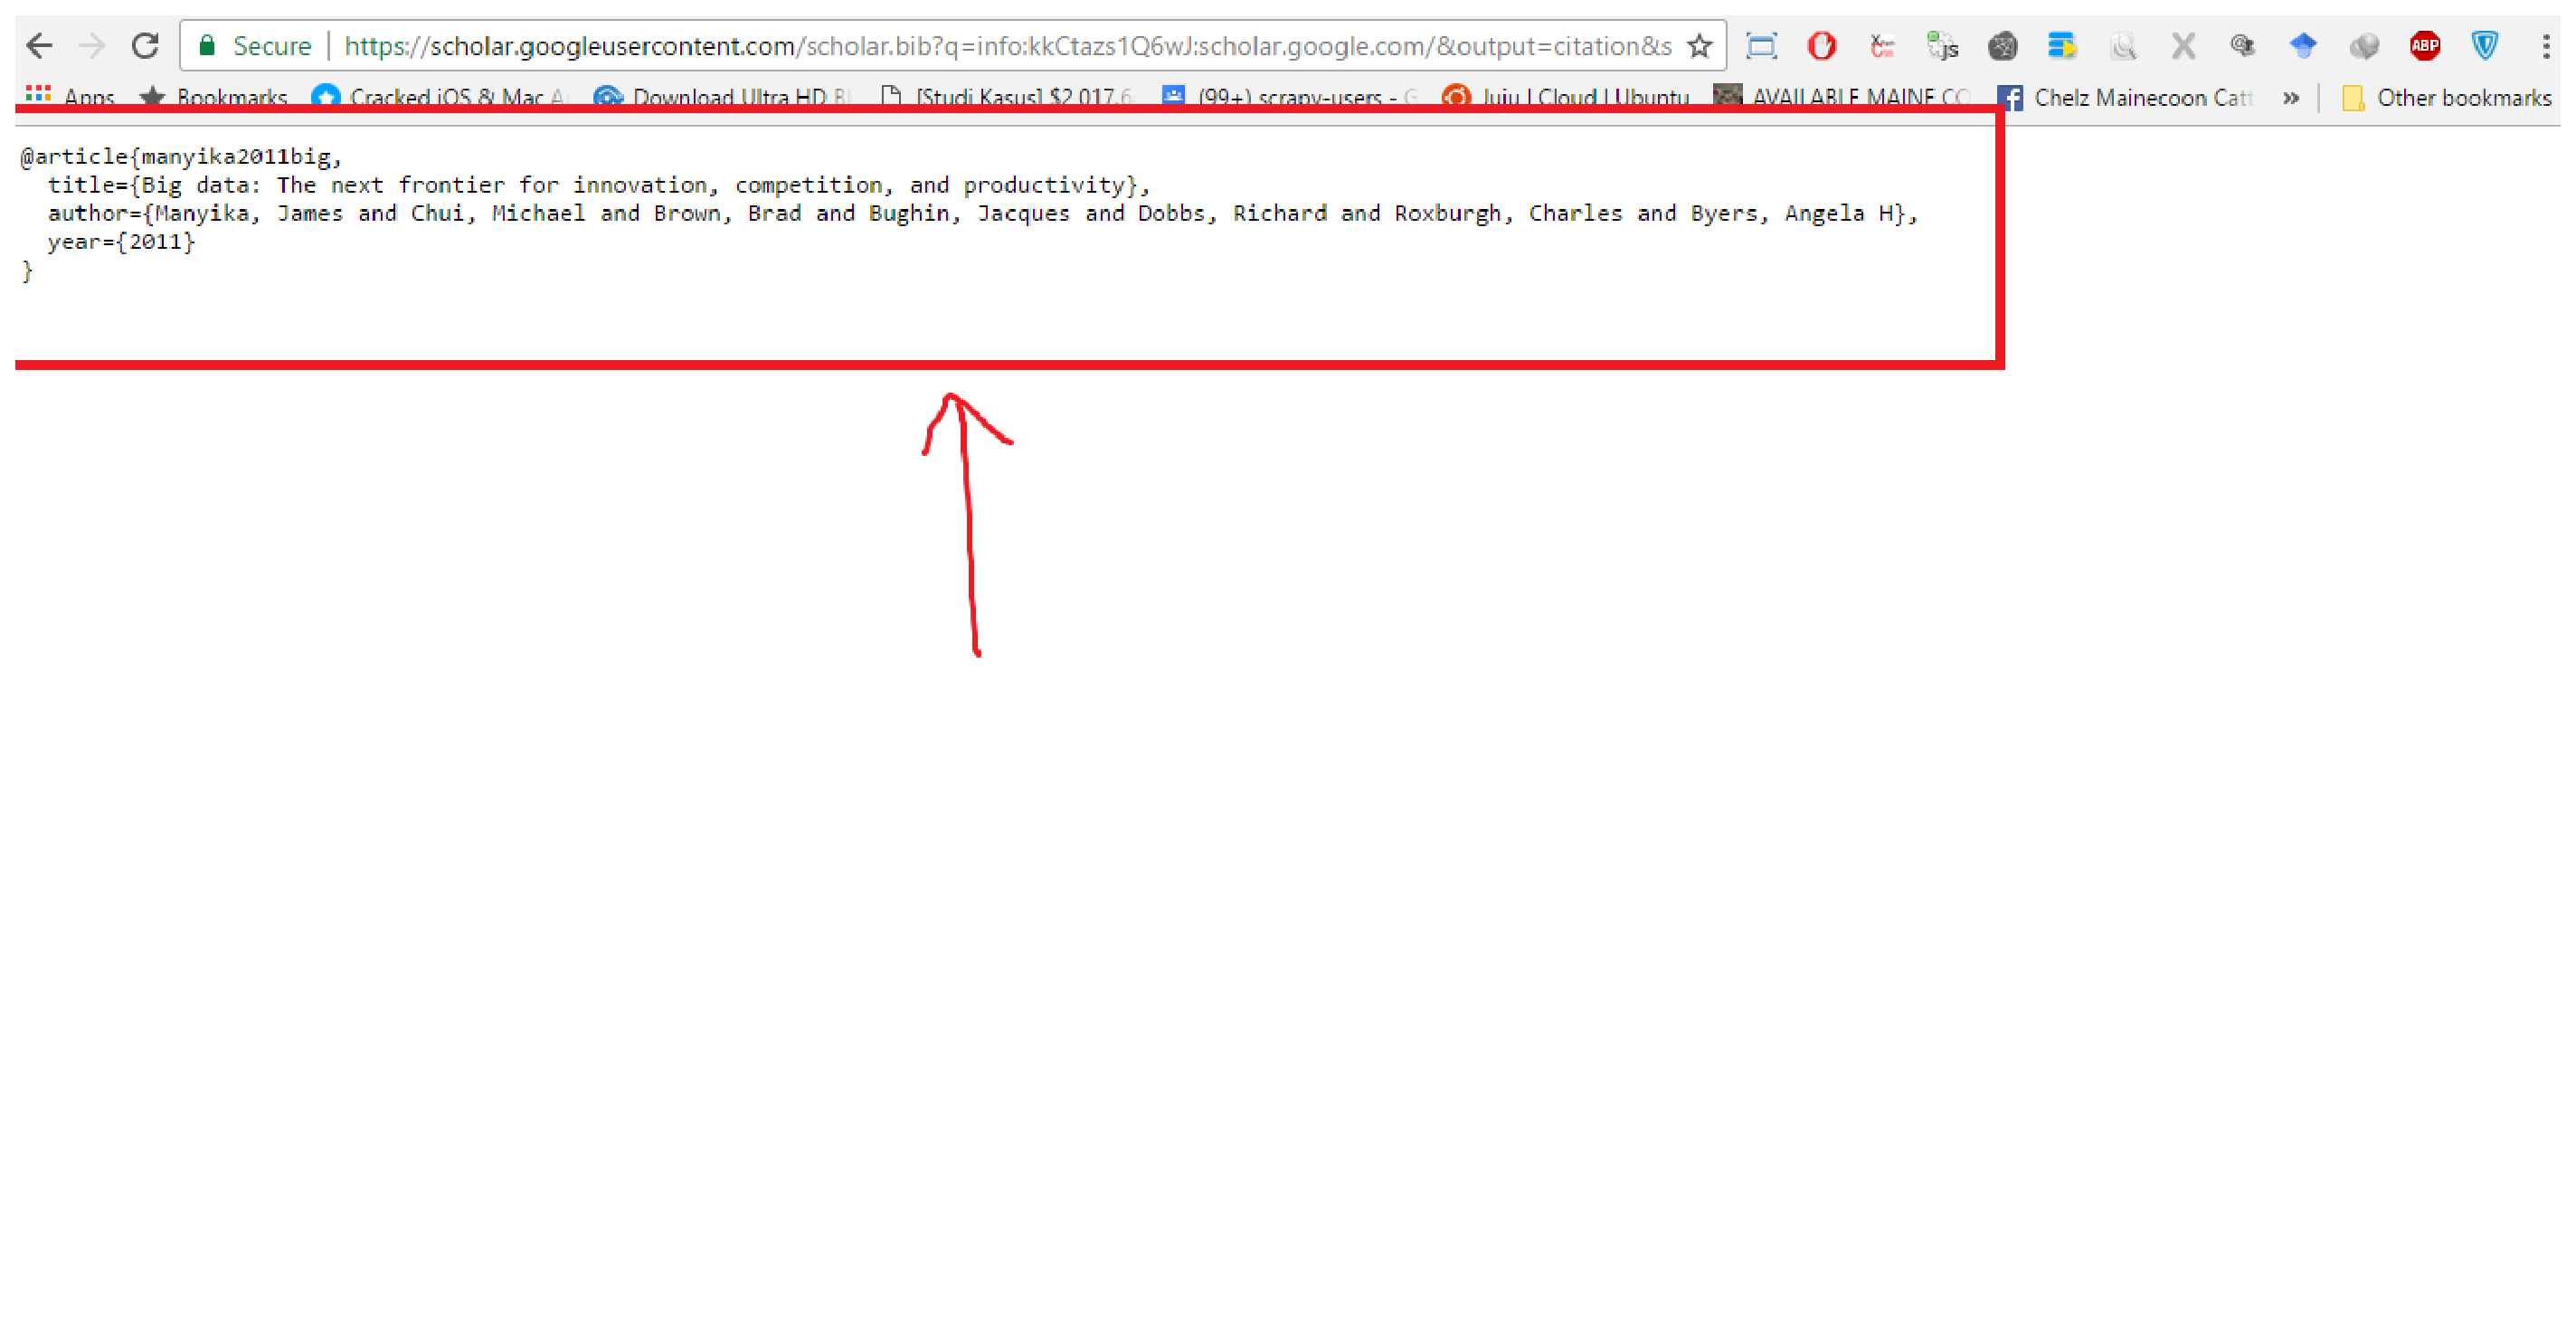
\includegraphics[width=120mm, height=120mm, keepaspectratio]{get_bib_script_part_4}
\caption{Copy the text}
\label{fig:fig3_4}
\end{figure}

For URL type references, you may check on one of my example of the $mybib.bib$ file. Once again, there are lots of alternative ways to write in LaTeX file.  % System Model

\section{Proposed Protocols}
Content goes here... 
 % Proposed Protocols
\chapter{Performance Evaluation}
\label{chap:simulation} 

Content goes here... 

\section{Simulation Setup}

Content goes here... 

\section{Simulation Results}

Content goes here...  % Performance Evaluation
\chapter{Conclusions and Future Directions}
\label{chap:conclsn}

\section{Conclusions}
Content goes here... 

\section{Future Directions}
See you again, hopefully it is useful for you guys! enjoy!
 % Conclusion and future work
\addcontentsline{toc}{chapter}{Bibliography}
%\begin{thebibliography}{99}

%\end{thebibliography}

%\bibliographystyle{unsrt}   % this means that the order of references
\bibliography{mybib}  % list here all the bibliographies that


\end{document}
